% Created 2017-09-08 Fri 07:30
\documentclass[11pt]{article}
\usepackage[utf8]{inputenc}
\usepackage[T1]{fontenc}
\usepackage{fixltx2e}
\usepackage{graphicx}
\usepackage{longtable}
\usepackage{float}
\usepackage{wrapfig}
\usepackage{rotating}
\usepackage[normalem]{ulem}
\usepackage{amsmath}
\usepackage{textcomp}
\usepackage{marvosym}
\usepackage{wasysym}
\usepackage{amssymb}
\usepackage{hyperref}
\tolerance=1000
\usepackage{ngerman}
\usepackage{amssymb}
\usepackage{amsmath}
\usepackage{tikz-qtree}
\usepackage{tikz}
\usetikzlibrary{matrix}
\author{Richard Stewing}
\date{\today}
\title{Zusammenfassung "Ubau}
\hypersetup{
  pdfkeywords={},
  pdfsubject={},
  pdfcreator={Emacs 25.2.1 (Org mode 8.2.10)}}
\begin{document}

\maketitle
\tableofcontents






\section{Weg zum generischen Compiler}
\label{sec-1}

\begin{itemize}
\item kontextfreie Sprache $\rightarrow$ Parser $\rightarrow$ Termalgebra $\rightarrow$ generische Faltung $\rightarrow$ Algebra
\end{itemize}

\section{Algebraische Modellierung}
\label{sec-2}

\subsection{Grundlagen}
\label{sec-2-1}

Seien A, B Mengen, f: A $\to$ B, C \subseteq A, D \subseteq B, n > 0.

\begin{itemize}
\item $\emptyset$: leere Menge
\item 1: \{$\epsilon$\}
\item 2: \{0,1\}
\item\relax [n]: \{1,..,n\}
\item $\Delta$$^{\text{n}}_{\text{A}}$ =$_{\text{def}}$ \{(a$_{\text{1}}$,..,a$_{\text{n}}$) $\in$ A$^{\text{n}}$ | $\forall$ 1 $\le$ i < n: a$_{\text{i}}$ = a$_{\text{i+1}}$ \}
\item f(C) =$_{\text{def}}$ \{f(a) | a $\in$ C\} = P(f)(C)
\item img(f) =$_{\text{def}}$ f(A)
\item f$^{\text{-1}}$(D) =$_{\text{def}}$ \{a $\in$ A | f(a) $\in$ D\}
\item ker(f) =$_{\text{def}}$ \{(a,a') $\in$ A \texttimes{} A | f(a) = f(a')\}
\item graph(f) =$_{\text{def}}$ \{(a, f(a)) $\in$ A \texttimes{} B | a $\in$ A\}
\item f|$_{\text{C}}$: C $\to$ B = c $\to$ f(c)
\item f[b/a]: A $\to$ B = c $\to$ if c = a then b else f(c)
\item $\chi$: P(A) $\to$ 2$^{\text{A}}$ = C $\to$ $\lambda$ a. if a $\in$ C then 1 else 0
\item f ist surjektiv $\Leftrightarrow$$_{\text{def}}$ img(f) = B
\item f ist injektiv $\Leftrightarrow$$_{\text{def}}$ ker(f) = $\Delta$$^{\text{2}}_{\text{A}}$
\item f ist bijektiv $\Leftrightarrow$$_{\text{def}}$ $\exists$ g: B $\to$ A: g . f = id$_{\text{A}}$ \and f . g = id$_{\text{B}}$
\item A $\cong$ B $\Leftrightarrow$$_{\text{def}}$ $\exists$ f: A $\to$ B und f ist bijektiv
\end{itemize}

\subsection{Mehrsortige Mengen}
\label{sec-2-2}

\begin{itemize}
\item Sei S eine Menge. Ein Tuple A = (A$_{\text{s}}$)$_{\text{s} \in \text{S}}$ ist dann eine S-indizierte(sortige) Menge.
\item Seien A = (A$_{\text{s}}$)$_{\text{s} \in \text{S}}$ und B = (B$_{\text{s}}$)$_{\text{s} \in\text{S}}$ S-sortige Mengen. f: A $\to$ B ist eine S-sortige Menge (f$_{\text{s}}$)$_{\text{s} \in \text{S}}$, so dass $\forall$ s $\in$ S. f$_{\text{s}}$:A$_{\text{s}}$ $\to$ B$_{\text{s}}$.
\item Seien n > 0. Eine n-stellige S-sortige Relation auf A ist eine S-sortige Menge R = (R$_{\text{s}}$)$_{\text{s} \in \text{S}}$ mit R$_{\text{s}}$ \subseteq A$_{\text{s}}^{\text{n}}$ f"ur alle  s$\in$ S.
\item Im Fall n = 1, hei"st R S-sortige Teilmenge von A genannt.
\item kartesisches Produkt einer I-sortigen Menge: \texttimes{}$_{\text{i} \in \text{I}}$A$_{\text{i}}$ = \{f:I $\to$ $\cup$$_{\text{i} \in\text{I}}$A$_{\text{i}}$ | $\forall$ i$\in$ I : f(i) $\in$ A$_{\text{i}}$\}
\item Gibt es eine Menge A mit A$_{\text{i}}$ = A f"ur alle i$\in$ I, dann stimmt \texttimes{}$_{\text{i} \in \text{I}}$A$_{\text{i}}$ offenbar mit A$^{\text{I}}$ "uberein. Im Fall I = [n] f"ur ein n > 1 schreibt man auch A$_{\text{1}}$ \texttimes{} \ldots{} \texttimes{} A$_{\text{n}}$ anstelle von \texttimes{}$_{\text{i} \in \text{I}}$ A$_{\text{i}}$ und A$^{\text{n}}$ snatelle von A$^{\text{I}}$.
\item disjunkte Vereinigung: \uplus$_{\text{i} \in \text{I}}$A$_{\text{i}}$ = $\cup$$_{\text{i} \in \text{I}}$(A$_{\text{i}}$ \texttimes{} \{i\})
\item Im Fall I = [n] f"ur ein n > 1 schreibt man auch A$_{\text{1}}$ + .. + A$_{\text{n}}$ anstelle von \uplus$_{\text{i} \in \text{I}}$A$_{\text{i}}$.
\item A$^{\text{+}}$ =$_{\text{def}}$ $\cup$$_{\text{n>0}}$A$^{\text{n}}$
\item 1 =$_{\text{def}}$ \{$\epsilon$\}
\item A$^{\text{*}}$ =$_{\text{def}}$ 1 $\cup$ A$^{\text{+}}$
\item $\cdot$: A$^{\text{*}}$ \texttimes{} A$^{\text{*}}$ $\to$ A$^{\text{*}}$ und $\cdot$: P(A$^{\text{*}}$) \texttimes{} P(A$^{\text{*}}$) $\to$ P(A$^{\text{*}}$) ist die Konkatenationen von Strings
\end{itemize}

\subsection{Produkte und Summen als universelle Konstruktionen}
\label{sec-2-3}

Sei I eine nichtleere Menge und A eine I-sortige Menge.
Das kartesische Produkt und die disjunkte Vereinigung eines Mengentupels A haben bestimmte \textbf{universelle Eigenschaften}.
\begin{itemize}
\item Jede Menge mit den universellen Eigenschaften des kartesischen Produkts nennt man \emph{Produkt von A}
\item Jede Menge mit den universellen Eigenschaften der disjunkten Vereinigung nennt man \emph{Summe von A}
\end{itemize}

\subsubsection{Produkt}
\label{sec-2-3-1}
Sei A = (A$_{\text{i}}$)$_{\text{i} \in \text{I}}$ ein Mengentuple, P eine Menge und $\pi$ = ($\pi$$_{\text{i}}$: P $\to$ A$_{\text{i}}$)$_{\text{i} \in \text{I}}$ ein Funktionstuple.
Das Paar (P, $\pi$) hei"st \textbf{Produkt von A}, wenn es f"ur alle Tuple (f$_{\text{i}}$: B $\to$ A$_{\text{i}}$)$_{\text{i} \in \text{I}}$ genau eine Funktion f: B $\to$ P gibt derart,
dass f"ur alle i$\in$ I Folgendes gilt:

\begin{center}
$\pi$$_{\text{i}}$ . f = f$_{\text{i}}$       
\end{center}

$\pi$$_{\text{i}}$ hei"st i-te Projektion von P und g Produktextension oder Range-Tuple von f. g wird mit \langle f$_{\text{i}}$ \rangle$_{\text{i} \in \text{I}}$ und im Falle
von I = [n], n > 1, auch mit \langle f$_{\text{1}}$,..,f$_{\text{n}}$ \rangle bezeichnet.

Demnach gilt:

\begin{center}
($\forall$ i$\in$ I : $\pi$$_{\text{i}}$ . f = $\pi$$_{\text{i}}$ \bigcirc g) $\Rightarrow$ f = g
\end{center}

\texttimes{}$_{\text{i} \in \text{I}}$A$_{\text{i}}$ ist ein Produkt von A.

Die Projektion und Produktextensionen f"ur \texttimes{}$_{\text{i} \in \text{I}}$A$_{\text{i}}$ sind wie folgt definiert:
\begin{itemize}
\item F"ur alle i$\in$ I und f$\in$ \texttimes{}$_{\text{i} \in \text{I}}$A$_{\text{i}}$, $\pi$$_{\text{i}}$(f) =$_{\text{def}}$ f(i)
\item F"ur alle (f$_{\text{i}}$: B $\to$ A$_{\text{i}}$)$_{\text{i} \in \text{I}}$, b$\in$ B und i $\in$ I, \langle f$_{\text{i}}$ \rangle$_{\text{i} \in \text{I}}$(b)(i) =$_{\text{def}}$ f$_{\text{i}}$(b).
\end{itemize}

\begin{enumerate}
\item Satz 2.2 Produkte sind \emph{bis auf Isomorphie} eindeutig:
\label{sec-2-3-1-1}
\begin{itemize}
\item Seien (P, $\pi$) und (P', $\pi$') Produkte von A. Dann sind P und P' isomorph.
\item Seien (P, $\pi$) ein Produkt von A, P' eine Menge und h: P' $\to$ P eine bijektive Abbildung. Dann ist (P', $\pi$') mit $\pi$' = ($\pi$ . h)$_{\text{i} \in \text{I}}$ ebenfalls ein Produkt von A.
\end{itemize}


Die Funktion 
\begin{center}
$\Pi$$_{\text{i} \in \text{I}}$f$_{\text{i}}$ =$_{\text{def}}$ \langle f$_{\text{i}}$ . $\pi$$_{\text{i}}$ \rangle : P $\to$ P'  
\end{center}
hei"st \textbf{Produkt von f}.

F"ur alle nichtleeren Mengen I,f: A $\to$ B und n > 0,

\begin{center}
f$^{\text{I}}$ =$_{\text{def}}$ $\Pi$$_{\text{i} \in \text{I}}$ f$_{\text{i}}$,  \\
f$_{\text{1}}$ \texttimes{} .. \texttimes{} f$_{\text{n}}$ =$_{\text{def}}$ $\Pi$$_{\text{i} \in \text{[n]}}$ f$_{\text{i}}$.
\end{center}

F"ur alle f: A $\to$ B, (f$_{\text{i}}$: B $\to$ B$_{\text{i}}$)$_{\text{i} \in \text{I}}$, (g$_{\text{i}}$: A$_{\text{i}}$ $\to$ B$_{\text{i}}$)$_{\text{i} \in \text{I}}$, k$\in$ I und (h$_{\text{i}}$: B$_{\text{i}}$ $\to$ A$_{\text{i}}$)$_{\text{i} \in \text{I}}$,
\begin{center}
\langle f$_{\text{i}}$ \rangle$_{\text{i} \in \text{I}}$ . f = \langle f$_{\text{i}}$ . f \rangle$_{\text{i} \in \text{I}}$, \\
$\pi$$_{\text{k}}$ . $\Pi$$_{\text{i} \in \text{I}}$g$_{\text{i}}$ = g$_{\text{k}}$ $\pi$$_{\text{k}}$, \\
($\Pi$$_{\text{i} \in \text{I}}$h$_{\text{i}}$) . \langle f$_{\text{i}}$ \rangle$_{\text{i} \in \text{I}}$ = \langle h$_{\text{i}}$ . f$_{\text{i}}$ \rangle$_{\text{i} \in \text{I}}$. \\
\end{center}
\end{enumerate}

\subsubsection{Summe}
\label{sec-2-3-2}

Vom Produkt kommt man zur Summe, indem man alle Funktionspfeile umdreht:
Sei A = (A$_{\text{i}}$)$_{\text{i} \in \text{I}}$ ein Mengentuple, S eine Menge und $\iota$ = ($\iota$$_{\text{i}}$: A$_{\text{i}}$ $\to$ S)$_{\text{i} \in \text{I}}$ ein Funktionstuple.
Das Paar (S, $\iota$) hei"st \textbf{Summe} oder \textbf{Coprodukt von A}, wenn es f"ur alle Tuple (f$_{\text{i}}$: A$_{\text{i}}$ $\to$ B)$_{\text{i} \in \text{I}}$ \uline{genau} eine Funktion
f: S $\to$ B gibt mit 
\begin{center}
f . $\iota$$_{\text{i}}$ = f$_{\text{i}}$
\end{center}
f"ur alle i $\in$ I. \\

$\iota$$_{\text{i}}$ hei"st i-te Injektion von S und g Summenextension oder Domain Tuplung von f. g wird mit [f$_{\text{i]}}$$_{\text{i} \in \text{I}}$ und im Falle I = [n],
n>1, auch mit [f$_{\text{1}}$,..,f$_{\text{n]}}$ bezeichnet. 

Demnach gilt:


\begin{center}
($\forall$ i$\in$ I : f . $\iota$$_{\text{i}}$ = g . $\iota$$_{\text{i}}$) $\Rightarrow$ f = g
\end{center}

\begin{enumerate}
\item Satz 2.3 Summen sind \emph{bis auf Isomorphie} eindeutig:
\label{sec-2-3-2-1}
\begin{itemize}
\item Seien (S, $\iota$) und (S', $\iota$') Summen von A. Dann sind P und P' isomorph.
\item Sei (S, $\iota$) eine Summe von A, S' eine Menge und h: S $\to$ S' eine bijektive Abbildung. Dann ist (S', $\iota$') mit $\iota$' = (h . $\iota$$_{\text{i}}$)$_{\text{i} \in \text{I}}$ ebenfalls eine summe von A.
\end{itemize}

Sei (S, $\iota$) eine Summe von (A$_{\text{i}}$)$_{\text{i} \in \text{I}}$, ein (S', $\iota$') eine Summe von (B$_{\text{i}}$)$_{\text{i} \in \text{I}}$ und f = (f$_{\text{i}}$: A$_{\text{i}}$ $\to$ B$_{\text{i}}$)$_{\text{i} \in \text{I}}$
Die Funktion
\begin{center}
\amalg$_{\text{i} \in \text{I}}$f$_{\text{i}}$ =$_{\text{def}}$ [$\iota$$_{\text{i}}$' . f$_{\text{i}}$]: S $\to$ S' 
\end{center}
hei"st Summe von f.


F"ur alle nichtleeren Mengen I,f: A $\to$ B und n>0,
\begin{center}
f \texttimes{} I =$_{\text{def}}$ \amalg$_{\text{i} \in \text{I}}$ f, \\
f$_{\text{1}}$+..+f$_{\text{n}}$ =$_{\text{def}}$ \amalg$_{\text{i} \in \text{[n]}}$ f$_{\text{i}}$, \\
f$^{\text{+}}$ =$_{\text{def}}$ \amalg$_{\text{n} \in \mathbb{N}}$ f$^{\text{[n]}}$, \\
f$^{\text{*}}$ =$_{\text{def}}$ 1 + f$^{\text{+}}$ =$_{\text{def}}$ id$_{\text{1}}$ + f$^{\text{+}}$. \\
\end{center}
\end{enumerate}

\subsection{Typen und Signaturen}
\label{sec-2-4}

Sei S eine Menge von - \textbf{Sorten} genannten - Symbolen.
Die Klasse T$_{\text{p}}$(S) der \textbf{polynomialen Typen "uber} S:
\begin{itemize}
\item S \subseteq T$_{\text{p}}$(S)
\item Jede nichtleere Menge ist ein polynomialer Typ
\item F"ur alle nichtleeren Mengen I und (e$_{\text{i}}$)$_{\text{i}\in\ \text{I}}$$\in$ T$_{\text{p}}$(S)$^{\text{I}}$, $\Pi$$_{\text{i}\in\ \text{I}}$ e$_{\text{i}}$, \amalg$_{\text{i}\in\ \text{I}}$e$_{\text{i}}$ $\in$ T$_{\text{p}}$(S)
\end{itemize}


\begin{itemize}
\item Ein Typ der Form $\Pi$$_{\text{i}\in\ \text{I}}$e$_{\text{i}}$ hei"st \textbf{I-stelliger Produkttyp} mit den \textbf{Faktoren} e$_{\text{i}}$, i$\in$ I.
\item Ein Typ der Form \amalg$_{\text{i}\in\ \text{I}}$e$_{\text{i}}$ hei"st \textbf{I-stelliger Summentyp} mit den \textbf{Summanden} e$_{\text{i}}$, i$\in$ I.
\end{itemize}

F"ur alle n>0, e$_{\text{1}}$,..,e$_{\text{n}}$, e$\in$ T$_{\text{p}}$(S) und nichtleere Mengen I,
\begin{center}
e$_{\text{1}}$ \texttimes{} .. \texttimes{} e$_{\text{n}}$ =$_{\text{def}}$ $\Pi$$_{\text{i} \in \text{[n]}}$e$_{\text{i}}$, \\
e$_{\text{1}}$ + .. + e$_{\text{n}}$ =$_{\text{def}}$ \amalg$_{\text{i} \in \text{[n]}}$e$_{\text{i}}$, \\
e$^{\text{I}}$ =$_{\text{def}}$ $\Pi$$_{\text{i} \in \text{I}}$e$_{\text{i}}$, \\
e$^{\text{n}}$ =$_{\text{def}}$ e$^{\text{[n]}}$, \\
e$^{\text{+}}$ =$_{\text{def}}$ \amalg$_{\text{n>0}}$e$^{\text{n}}$, \\
e$^{\text{*}}$ =$_{\text{def}}$ 1 + e$^{\text{+}}$. \\
\end{center}

Eine S-sortige Menge A wird wie folgt zur T$_{\text{p}}$(S)-sortigen Menge erweitert: F"ur alle nichtleeren Mengen I und (e$_{\text{i}}$)$_{\text{i} \in \text{I}}$

\begin{center}
A$_{\text{I}}$ = I, \\
A$_{\Pi_{\text{i} \in \text{I}}\text{e}_{\text{i}}}$ = \texttimes{}$_{\text{i} \in \text{I}}$ A$_{\text{e}_{\text{i}}}$, \\
A$_{\amalg_{\text{i} \in \text{I}}\text{e}_{\text{i}}}$ = \uplus$_{\text{i} \in \text{I}}$ A$_{\text{e}_{\text{i}}}$.
\end{center}

F"ur alle e $\in$ T$_{\text{p}}$(S) und a $\in$ A$_{\text{e}}$ nennen wir e den Typen von a.

Eine S-sortige Funktion h: A $\to$ B wird wie folgt zur T$_{\text{p}}$(S)-sortigen Menge f"ur alle nichtleeren Mengen I und (e$_{\text{i}}$)$_{\text{i } \in }$ 
$\in$ T$_{\text{p}}$(S)$^{\text{I}}$.

\begin{center}
h$_{\text{I}}$ = id$_{\text{I}}$, \\
h$_{\Pi_{\text{i } \in \text{I}}}$ = $\Pi$$_{\text{i} \in \text{I}}$h$_{\text{e}_{\text{i}}}$, \\
h$_{\amalg_{\text{i } \in \text{I}}}$ = \amalg$_{\text{i} \in \text{I}}$h$_{\text{e}_{\text{i}}}$.
\end{center}


F"ur alle S-sortigen Mengen A, S-sortige Funktionen h: A $\to$ B, n>0, nichtleeren Menge I und e$_{\text{1}}$,..e$_{\text{n}}$, e $\in$ T$_{\text{p}}$(S) gilt Folgendes:
\begin{center}
A$_{\text{e}_{\text{1}} \ \texttimes{}\ \text{.. }\texttimes{}\ \text{e}_{\text{n}}}$ = A$_{\text{e}_{\text{1}}}$ \texttimes{} .. \texttimes{} A$_{\text{e}_{\text{n}}}$, \\
A$_{\text{e}_{\text{1}} \ \text{+ .. + e}_{\text{n}}}$ = A$_{\text{e}_{\text{1}}}$ + .. + A$_{\text{e}_{\text{n}}}$, \\
A$_{\text{e}^{\text{I}}}$ = A$^{\text{I}}_{\text{e}}$, \\
A$_{\text{e}^{\text{n}}}$ = A$^{\text{n}}_{\text{e}}$, \\
A$_{\text{e}^{\text{+}}}$ = A$^{\text{+}}_{\text{e}}$, \\
A$_{\text{e}^{\text{*}}}$ = A$^{\text{*}}_{\text{e}}$, \\

h$_{\text{e}_{\text{1}} \ \texttimes{}\ \text{.. }\texttimes{}\ \text{e}_{\text{n}}}$ = h$_{\text{e}_{\text{1}}}$ \texttimes{} .. \texttimes{} h$_{\text{e}_{\text{n}}}$, \\
h$_{\text{e}_{\text{1}} \ \text{+ .. + e}_{\text{n}}}$ = h$_{\text{e}_{\text{1}}}$ + .. + h$_{\text{e}_{\text{n}}}$, \\
h$_{\text{e}^{\text{I}}}$ = h$^{\text{I}}_{\text{e}}$, \\
h$_{\text{e}^{\text{n}}}$ = h$^{\text{[n]}}_{\text{e}}$, \\
h$_{\text{e}^{\text{+}}}$ = h$^{\text{+}}_{\text{e}}$, \\
h$_{\text{e}^{\text{*}}}$ = h$^{\text{*}}_{\text{e}}$.
\end{center}



\subsection{Signaturen}
\label{sec-2-5}

\begin{itemize}
\item Eine \textbf{Signatur} $\Sigma$ = (S, F) besteht aus einer Menge S von Sorten wie oben sowie einer Menge F typisierter Funktionssymbole f: e $\to$ e' mit e, e' $\in$ T$_{\text{p}}$(S), den Operationen von $\Sigma$.
\item obs($\Sigma$): die Menge der \textbf{beobachtbaren Typen} (observable types) von $\Sigma$, das sind alle nichtleeren Mengenm die in Typen von Operationen von $\Sigma$ vorkommen.
\item $\forall$ f$\in$ F : f: e $\to$ e', dom(f) = e und ran(f) = e'
\item $\Sigma$ hei"st \textbf{Gentzen-Signatur}, falls $\forall$ f $\in$ F Mengen I, J existieren sodass dom(f) ein I-stelliger Produkttyp und ran(f) ein J-stelliger Summentyp ist.
\item Konsrtuktoren dienen der Synthese von Elementen einer S-sortigen Menge, Destruktoren liefern Werkzeuge zu ihrer Analyse.
\item Abstrakte Syntax einer CFG ist eine konstruktive Signaturen
\item Parser, Interpreter und Compiler beruhen auf Automatenmodelle, die destruktive Signaturen interpretieren
\end{itemize}

\subsubsection{Konstruktive Signaturen}
\label{sec-2-5-1}

\begin{enumerate}
\item Mon ($\Rightarrow$ Unmarkierte bin"are B"aume)
\label{sec-2-5-1-1}
\begin{itemize}
\item S = \{mon\}
\item F = \{one: 1 $\to$ mon, mul: mon \texttimes{} mon $\to$ mon\}
\end{itemize}

\item Nat ($\Rightarrow$ N)
\label{sec-2-5-1-2}
\begin{itemize}
\item S = \{nat\}
\item F = \{zero: 1 $\to$ nat, succ: nat $\to$ nat\}
\end{itemize}

\item Dyn(I, X) ($\Rightarrow$ I \texttimes{} X$^{\text{*}}$)
\label{sec-2-5-1-3}
\begin{itemize}
\item S = \{list\}
\item F = \{nil: I $\to$ list. cons: X \texttimes{} list $\to$ list\}
\end{itemize}

\item List(X) =$_{\text{def}}$ Dyn(1, X) ($\Rightarrow$ X$^{\text{*}}$)
\label{sec-2-5-1-4}

\item Bintree(X) ($\Rightarrow$ bin"are B"aume endlicher Tiefe mit Knotenmarkierungen aus X)
\label{sec-2-5-1-5}
\begin{itemize}
\item S = \{btree\}
\item F = \{empty: 1 $\to$ btree, bjoin: btree \texttimes{} X \texttimes{} btree $\to$ btree\}
\end{itemize}


\item Tree(X) ($\Rightarrow$ B"aume endlicher Tiefe und endlichen Knotenausgrads mit Knotenmarkierungen aus X)
\label{sec-2-5-1-6}
\begin{itemize}
\item S = \{tree, trees\}
\item F = \{join: X \texttimes{} trees $\to$ tree, nil: 1 $\to$ trees, cons: tree \texttimes{} trees $\to$ trees\}
\end{itemize}

\item Reg(BL) ($\Rightarrow$ regul"are Ausdr"ucke "uber BL)
\label{sec-2-5-1-7}
\begin{itemize}
\item S = \{reg\}
\item F = \{par: reg \texttimes{} reg $\to$ reg, seq: reg \texttimes{} reg $\to$ reg, iter: reg $\to$ reg, base: BL $\to$ reg\}
\end{itemize}

\item CCS(Act) ($\Rightarrow$ Calculus of Communicating Systems)
\label{sec-2-5-1-8}
\begin{itemize}
\item S = \{proc\}
\item F = \{ pre: Act \texttimes{} proc $\to$ proc, cho: proc \texttimes{} proc $\to$ proc, par: proc \texttimes{} proc $\to$ proc, res: proc \texttimes{} Act $\to$ proc, rel: proc \texttimes{} Act$^{\text{Act}}$ $\to$ proc\}
\end{itemize}
\end{enumerate}


\subsubsection{Destruktive Signaturen}
\label{sec-2-5-2}

\begin{enumerate}
\item coNat ($\Rightarrow$ N $\cup$ \{$\infty$\})
\label{sec-2-5-2-1}
\begin{itemize}
\item S = \{nat\}
\item F = \{pred: nat $\to$ 1 + nat\}
\end{itemize}

\item coList(X) ($\Rightarrow$ X$^{\text{*}}$ $\cup$ X$^{\text{N}}$ (coList(1) $\cong$ coNat))
\label{sec-2-5-2-2}
\begin{itemize}
\item S = \{list, X \texttimes{} list\}
\item F = \{split: list $\to$ 1+ X \texttimes{} list, $\pi$$_{\text{1}}$: X \texttimes{} list $\to$ X, $\pi$$_{\text{2}}$: X \texttimes{} list $\to$ list\}
\end{itemize}

\item Stream(X) =$_{\text{def}}$ DAut(1, X) ($\Rightarrow$ X$^{\text{N}}$)
\label{sec-2-5-2-3}
\begin{itemize}
\item S = \{list\}
\item F = \{head: list $\to$ X, tail: list $\to$ list\}
\end{itemize}

\item coBintree(X) ($\Rightarrow$ bin"are B"aume beliebiger Tiefe mit Knotenmarkierungen aus X)
\label{sec-2-5-2-4}
\begin{itemize}
\item S = \{btree, btree \texttimes{} X \texttimes{} btree\}
\item F = \{split: btree $\to$ 1 + btree \texttimes{} X \texttimes{} btree, $\pi$$_{\text{1}}$: btree \texttimes{} X \texttimes{} btree $\to$ btree, $\pi$$_{\text{2}}$: btree \texttimes{} X \texttimes{} btree $\to$ X, $\pi$$_{\text{3}}$: btree \texttimes{} X \texttimes{} btree $\to$ btree\}
\end{itemize}

\item Infbintree(X) ($\Rightarrow$ bin"are B"aume unendlicher Tiefe mit Knotenmarkierungen aus X)
\label{sec-2-5-2-5}
\begin{itemize}
\item S = \{btree\}
\item F = \{root: btree $\to$ X, left, right:btree $\to$ btree\}
\end{itemize}

\item DAut(X,Y) ($\Rightarrow$ Y$^{\text{X}^{\text{*}}}$ = Verhalten det. Moore-Automaten mit Eingabemenge X und Ausgabemenge Y)
\label{sec-2-5-2-6}
\begin{itemize}
\item S = \{state, state$^{\text{X}}$\}
\item F = \{$\delta$: state $\to$ state$^{\text{X}}$, $\beta$: state $\to$ Y\} $\cup$ \{$\pi$$_{\text{x}}$: state$^{\text{X}}$ $\to$ state | x$\in$ X\}
\end{itemize}

\item Acc(X) =$_{\text{def}}$ DAut(X,2) ($\Rightarrow$ P(X$^{\text{*}}$) = Wortsprache "uber X)
\label{sec-2-5-2-7}

\item Proctree(Act) ($\Rightarrow$ Prozessb"aume, deren Kanten mit Aktionen markiert sind)
\label{sec-2-5-2-8}
\begin{itemize}
\item S = \{tree\} $\cup$ \{(Act \texttimes{} tree)$^{\text{n}}$ | n > 0\}
\item F = \{$\delta$: tree $\to$ (Act \texttimes{} tree)$^{\text{*}}$\} $\cup$ \{$\pi$$_{\text{n}}$: (Act \texttimes{} tree)$^{\text{n}}$ $\to$ Act \texttimes{} tree | n > 0\} $\cup$ \{$\pi$$_{\text{1}}$: Act \texttimes{} tree $\to$ Act, $\pi$$_{\text{2}}$: Act \texttimes{} tree $\to$ tree\}
\end{itemize}
\end{enumerate}

\subsection{Algebren}
\label{sec-2-6}

Sei $\Sigma$ = (S, F) eine Signatur. Eine $\Sigma$- \textbf{Algebra} A = (A, Op) besteht aus einer S-sortigen Menge A und einer F-sortigen Menge
\begin{center}
Op = (f$^{\text{A}}$: A$_{\text{e}}$ $\to$ A$_{\text{e'}}$)$_{\text{f: e} \to \text{e'} \in \text{F}}$
\end{center}
von Funktionen, den Operationen von A.
F"ur alle s $\in$ S hei"st A$_{\text{s}}$ Tr"agermenge (carrier set) oder Interpretation von s in A. F"ur alle f: e $\to$ e' $\in$ F hei"st f$^{\text{A}}$ : A$_{\text{e}}$ $\to$ A$_{\text{e'}}$ Interpreation von f in A.

Seien A, B $\Sigma$-Algebren. Eine S-sortige Funktion h: A $\to$ B hei"st $\Sigma$-Homomorphismus, wenn f"ur alle f: e $\to$ e' $\in$ F
\begin{center}
h$_{\text{e'}}$ \bigcirc f$^{\text{A}}$ = f$^{\text{B}}$ \bigcirc h$_{\text{e}}$
\end{center}
gilt. Ist h bijektiv, dann hei"st h $\Sigma$-Isomorphismus und A und B sind $\Sigma$-isomorph. h induziert die Bildalgebra h(A):
\begin{itemize}
\item F"ur alle e$\in$ T$_{\text{p}}$(S), h(A)$_{\text{e}}$ =$_{\text{def}}$ h$_{\text{e}}$(A$_{\text{e}}$)
\item F"ur alle f: e$\to$ e' $\in$ F und a $\in$ A$_{\text{e}}$, f$^{\text{h(A)}}$(h(a)) =$_{\text{def}}$ f$^{\text{B}}$(h(a))
\end{itemize}

\subsubsection{Beispiele}
\label{sec-2-6-1}

\begin{enumerate}
\item Nat-Algebra
\label{sec-2-6-1-1}
\begin{itemize}
\item zero$^{\text{N}}$: 1 $\to$ N, succ$^{\text{N}}$: N $\to$ N
\item zreo$^{\text{N}}$($\epsilon$) = 0, succ$^{\text{N}}$(n) = n + 1
\end{itemize}

\item Word(X) (eine Mon-Algebra)
\label{sec-2-6-1-2}
\begin{itemize}
\item one$^{\text{Word(X)}}$: 1 $\to$ X$^{\text{*}}$, mul$^{\text{Word(X)}}$: X$^{\text{*}}$ \texttimes{} X$^{\text{*}}$ $\to$ X$^{\text{*}}$
\item one$^{\text{Word(X)}}$($\epsilon$) = $\epsilon$, mult$^{\text{Word(X)}}$(u, v) = uv
\end{itemize}
\end{enumerate}


\subsection{Terme und Coterme}
\label{sec-2-7}
\subsubsection{Terme}
\label{sec-2-7-1}
Sei $\Sigma$ = (S,C) eine konstruktive Signatur, X = $\cup$ obs($\Sigma$) und V eine S-sortige Menge von "Variablen".
Die Menge CT$_{\Sigma}$(V) der $\Sigma$-Terme "uber V ist die gr"o"ste (S $\cup$ obs($\Sigma$))-sortige Menge M  det. B"aume "uber (X, C $\cup$ X $\cup$ V)
mit folgenden Eigenschaften:

\begin{itemize}
\item F"ur alle B $\in$ obs($\Sigma$), M$_{\text{B}}$ = B (1)
\item F"ur alle s $\in$ S und t $\in$ M$_{\text{s}}$ ist t $\in$ V$_{\text{s}}$ (2) oder gibt es c: $\Pi$$_{\text{i} \in \text{I}}$s$_{\text{i}}$ $\to$ s $\in$ C und (t$_{\text{i}}$)$_{\text{i} \in \text{I}}$ $\in$ \texttimes{}$_{\text{i} \in \text{I}}$M$_{\text{s}_{\text{i}}}$ mit t = c\{i $\to$ t$_{\text{i}}$ | i $\in$ I\} (3)
\end{itemize}




\begin{enumerate}
\item Fall
\label{sec-2-7-1-1}
\\ 
\Tree [.b ] \\
b $\in$ B, 
B $\in$ obs($\Sigma$) \\

\item Fall
\label{sec-2-7-1-2}
\\
\Tree [.x ] \\
x ist von s, s $\in$ S, x $\in$ V$_{\text{s}}$ 

\item Fall
\label{sec-2-7-1-3}
\\
\Tree [.c \ldots \\
          \ldots \\
          \ldots \\
          [.i s$_{\text{i}}$ ]
          \ldots \\ ]

c: $\Pi$$_{\text{i} \in \text{I}}$ s$_{\text{i}}$ $\to$ s $\in$ C


\begin{itemize}
\item Die Elemente von CT$_{\Sigma}$ =$_{\text{def}}$ CT$_{\Sigma}$($\lambda$ x. $\emptyset$) hei"sen $\Sigma$-Grundterme.
\end{itemize}
\end{enumerate}

\subsubsection{Coterme}
\label{sec-2-7-2}
Sei $\Sigma$ = (S, D) eine destruktive Signatur und V eine S-sortige Menge von Farbe oder Covariablen.

Die Menge DT$_{\Sigma}$(V) der $\Sigma$-Coterme "uber V ist die gr"o"ste Menge (S $\cup$ obs($\Sigma$))-sortige Menge M det. B"aume "uber (D $\cup$ \{!\}, X $\cup$ V) mit (1) und folgender Eigenschaft
\begin{itemize}
\item F"ur alle s $\in$ S, t $\in$ M$_{\text{s}}$, d: s $\to$ \amalg$_{\text{i} \in \text{I}}$s$_{\text{i}}$ $\in$ D gibt es x $\in$ V$_{\text{s}}$, i$_{\text{d}}$ $\in$ I und t$_{\text{d}}$ $\in$ M$_{\text{s}_{\text{i}}}$ mit t =x\{d $\to$ i\{! $\to$ t$_{\text{d}}$\} | d: s $\to$ e $\in$ D\}
\end{itemize}

\begin{enumerate}
\item Fall
\label{sec-2-7-2-1}
\\ 
\Tree [.b ] \\
b $\in$ B, 
B $\in$ obs($\Sigma$) \\

\item Fall
\label{sec-2-7-2-2}
\\
\Tree [.x \ldots \\
          \ldots \\
          \ldots \\
          [.i s$_{\text{i}}$ ]
          \ldots \\ ]

x $\in$ V$_{\text{s}}$
c: s $\to$ \amalg$_{\text{i} \in \text{I}}$ s$_{\text{i}}$  $\in$ D

Ist I einelementig, dann stimmt \amalg$_{\text{i} \in \text{I}}$s$_{\text{i}}$ mit s$_{\text{i}}$ "uberein, so dass die mit ! markierte Kante entf"allt.
\end{enumerate}

\subsection{\emph{Bool}-Algebra}
\label{sec-2-8}
Die Menge 2 ist Tr"agermenge der REG(BL)-Algebra \emph{Bool}.

F"ur alle x, y $\in$ 2 und B $\in$ BL $\backslash$ 1:
\begin{center}
par$^{\text{Bool}}$(x, y) = max\{x,y\}, \\
seq$^{\text{Bool}}$(x, y) = x*y, \\
iter$^{\text{Bool}}$(x) = 1, \\
base$^{\text{Bool}}$(1) = 1, \\
bas$^{\text{Bool}}$(B) = 0. \\
\end{center}


\subsection{Termfaltung}
\label{sec-2-9}
\begin{itemize}
\item $\Sigma$ = (S, C)
\item V eine S-sortige Menge
\item A = (A, Op) eine $\Sigma$-Algebra
\item g: V $\to$ A eine \textbf{Variablenbelegung} (\emph{valuation})
\item g$^{\text{*}}$ intuitiv definiert.
\end{itemize}


Offenbar h"angt die Einschr"ankung von g* auf Grundterme nicht von g ab. Sie wird \textbf{Termfaltung} genannt und mit fold$^{\text{A}}$ bezeichnet.

Folglich ist fold$^{\text{A}}$ der einzige $\Sigma$-Homomorphismus von T$_{\Sigma}$ nach A

\subsection{Zustandsentfaltung}
\label{sec-2-10}
\begin{itemize}
\item $\Sigma$ = (S, D)
\item V eine S-sortige Menge
\item A = (A, Op) eine $\Sigma$-Algebra
\item g: A $\to$ V eine F"arbung
\item g$^{\text{\#}}$ intuitiv definiert
\end{itemize}

Offenbar h"angt die Einschr"ankung von g$^{\text{\#}}$ auf Grundterme nicht von g ab. Sie wird \textbf{Zustandsentfaltung} genannt und mit unfold$^{\text{A}}$ bezeichnet.

\section{Rechnen mit Algebren}
\label{sec-3}

\subsection{Unteralgebra}
\label{sec-3-1}
Bez"uglich der Operationen geschlossene Untermenge.

\subsection{Substitution}
\label{sec-3-2}
$\sigma$$^{\text{*}}$: T$_{\Sigma}$(V) $\to$ T$_{\Sigma}$(V)

\subsection{Term"aquivalenz}
\label{sec-3-3}
$\forall$ t,t' $\in$ E, g $\in$ A$^{\text{V}}$ : g$^{\text{*}}$(t) = g$^{\text{*}}$(t')


\subsection{Normalformen}
\label{sec-3-4}
Werden f"ur jede Signatur selbst definiert und k"onnen durch das verwenden definierter Gleichungen erzeugt Werden

\section{Kontextfreie Grammatiken (CFGs)}
\label{sec-4}

\subsection{Definition}
\label{sec-4-1}
G = (S, BS, R) mit 

\begin{itemize}
\item einer endlichen Menge S von \textbf{Sorten}, die auch Nichtterminale oder Variablen genannt werden
\item BS, eine Menge nichtleerer Basismengen
\item eine endliche Menge R von Regeln s $\to$ w mit s $\in$ S und \\ w $\in$ (S $\cup$ BS)$^{\text{*}}$ $\backslash$ \{s\}
\end{itemize}

\subsection{Die JavaLight Grammatik}
\label{sec-4-2}
\subsubsection{R}
\label{sec-4-2-1}
\begin{itemize}
\item Commands $\to$ Command Commands | Command
\item Command $\to$ \{Commands\} | String = Sum; | \\ if Disjunct Command else Command | \\ if Disjunct Command | while Disjunct Command
\item Sum $\to$ Sum + Prod | Sum - Prod | Prod
\item Prod $\to$ Prod * Factor | Prod/Factor | Factor
\item Factor $\to$ Z | String | (Sum)
\item Disjunct $\to$ Conjunct || Disjunct | Conjunct
\item Conjunct $\to$ Literal \&\& Conjunct | Literal
\item Literal $\to$ !Literal | Sum Rel Sum | 2 | (Disjunct)
\end{itemize}

\subsubsection{BS}
\label{sec-4-2-2}
\begin{itemize}
\item String (alle Zeichenfolgen au"ser Elementen anderer Basismengen von JavaLight)
\item Z
\item Rel (nicht n"aher spezifizierter bin"arer Relationen auf Z
\end{itemize}

\subsection{Beispiel Programm}
\label{sec-4-3}

fact = 1; while x > 1 \{fact = fact*x; x = x-1;\}

\subsection{Linksrekursive Grammatiken}
\label{sec-4-4}

Sei G = (S, BS, R) und X = $\cup$ BS. 

X ist die Menge der Eingabesymbole, die Compiler f"ur G verarbeiten m"ussen.

\subsubsection{Einschub Ableitungsrelation}
\label{sec-4-4-1}
$\to$$_{\text{G}}$ = \{(vsw, v$\alpha$ w), s $\to$ $\alpha$ $\in$ R, v,w $\in$ (S $\cup$ BS)$^{\text{*}}$\}.


\subsubsection{Definition}
\label{sec-4-4-2}
\begin{itemize}
\item G hei"st \textbf{linksrekursiv}, falls es eine \textbf{linkrekursive} Ableitung s $\to$$_{\text{G}}$ sv gibt.
\item G hei"st LL-kompilierbar, falls es eine partielle Ordnung $\le$ auf S gibt mit s' $\le$ s f"ur alle Ableitungen sv $\to$$_{\text{G}}$ s'w
\end{itemize}
\begin{enumerate}
\item Umgangssprachlich
\label{sec-4-4-2-1}
Man hat eine Regel, sodass die Sorte auf der linken Seite auf der rechten Seite ganz links vorkommt.
\end{enumerate}

\subsubsection{Beispiel}
\label{sec-4-4-3}
Z.B. REG ist LL-kompilierbar, JavaLight jedoch \uline{nicht}. 

\subsubsection{Verfahren zur Elemenierung von Linksrekursion}
\label{sec-4-4-4}
Sei G = (S, BS, R) und S = \{s$_{\text{1}}$,..,s$_{\text{n}}$\}.

F"uhre f"ur alle 1 $\le$ i $\le$ n die beiden folgenden Schritte in der angegebenen Reihenfolge durch:

\begin{itemize}
\item F"ur alle 1 $\le$ j $\le$ i und Regelpaare (s$_{\text{i}}$ $\to$ s$_{\text{j}}$v, s$_{\text{j}}$ $\to$ w) ersetze dir Regel s$_{\text{i}}$ $\to$ s$_{\text{j}}$v durch s$_{\text{i}}$ $\to$ wv
\item Falls vorhanden, streiche die Regel s$_{\text{i}}$ $\to$ s$_{\text{i}}$
\item F"ur alle Regelpaare (s$_{\text{i}}$ $\to$ v, s$_{\text{i}}$ $\to$ s$_{\text{i}}$w) mit $\notin$ \{s$_{\text{i}}$\} \texttimes{} (S $\cup$ BS)$^{\text{*}}$ ersetze die beiden Regeln durch die drei neuen Regeln s$_{\text{i}}$ $\to$ vs'$_{\text{i}}$, s'$_{\text{i}}$ $\to$ ws'$_{\text{i}}$ und s'$_{\text{i}}$ $\to$ $\epsilon$
\end{itemize}


\begin{enumerate}
\item Beispiel JavaLight
\label{sec-4-4-4-1}

\begin{itemize}
\item Commands $\to$ Command Commands | Command
\item Command $\to$ \{Commands\} | String = Sum; | \\ if Disjunct Command else Command | \\ if Disjunct Command | while Disjunct Command
\item Sum $\to$ Prod Sumsect
\item Sumsect $\to$ + Prod Sumsect | - Prod Sumsect | $\epsilon$
\item Prod $\to$ Factor Prodsect
\item Prodsect $\to$ * Factor Prodsect | / Factor Prodsect | $\epsilon$
\item Factor $\to$ Z | String | (Sum)
\item Disjunct $\to$ Conjunct || Disjunct | Conjunct
\item Conjunct $\to$ Literal \&\& Conjunct | Literal
\item Literal $\to$ !Literal | Sum Rel Sum | 2 | (Disjunct)
\end{itemize}
\end{enumerate}



\subsection{Abstrakte Syntax}
\label{sec-4-5}

Sei G = (S, BS, R) eine CFG.

Die folgende Funktion typ: (S $\cup$ BS)$^{\text{*}}$ $\to$ T$_{\text{p}}$(S) streicht alle Elemente von Z(G) aus W"ortern "uber S $\cup$ BS und "uberf"uhrt diese
in die durch sie bezeichneten Produkttypen:

\begin{itemize}
\item typ($\epsilon$) = 1
\item F"ur alle s $\in$ S $\cup$ BS $\backslash$ Z(G) und w $\in$ (S $\cup$ BS)$^{\text{*}}$, typ(sw) = s \texttimes{} typ(w)
\item F"ur alle x $\in$ Z und w $\in$ (S $\cup$ BS)$^{\text{*}}$, typ(xw) = typ(w)
\end{itemize}

Dann ist $\Sigma$(G) = (S, BS, \{f$_{\text{s }\to\ \text{w}}$:typ(w) $\to$ s | s $\to$ w $\in$ R\})


$\Sigma$(G)-Grundterme werden Syntaxb"aume von G genannt.

\subsubsection{Beispiel JavaLight}
\label{sec-4-5-1}
\begin{itemize}
\item S = \{Commands, Command, Sum, Prod, Factor, Disjunct, Conjunct, Literal\}
\item I = \{Z, String, Rel, 2\}
\item F = \{ \\ seq: Command \texttimes{} Commands $\to$ Commands, \\ embed: Command $\to$ Commands, \\ block: Commands $\to$ Command, \\ assign: String \texttimes{} Sum $\to$ Command, \\ cond: Disjunct \texttimes{} Command \texttimes{} Command $\to$ Command, \\ cond1, loop: Disjunct \texttimes{} Command $\to$ Command, \\ \uline{sum}: Prod $\to$ Sum, \\ \uline{plus}, \uline{minus}: Sum \texttimes{} Prod $\to$ Sum, \\ \uline{prod}: Factor $\to$ Prod, \\ \uline{times}, \uline{div}: Prod \texttimes{} Factor $\to$ Prod, \\ embedI: Z $\to$ Factor, \\ var: String $\to$ Factor, \\ encloseS: Sum $\to$ Factor, \\ disjunct: Conjunct \texttimes{} Disjunct $\to$ Disjunct, \\ embedC: Conjunct $\to$ Disjunct, \\ conjunct: Literal \texttimes{} Conjunct $\to$ Conjunct, \\ embedL: Literal $\to$ Conjunct, \\ not: Literal $\to$ Literal, \\ atom: Rel \texttimes{} Sum \texttimes{} Sum $\to$ Literal, \\ embedB: 2 $\to$ Literal, \\ encloseD: Disjunct $\to$ Literal\}
\end{itemize}


\subsubsection{JavaLight' (entlinksrekursiv)}
\label{sec-4-5-2}
\begin{itemize}
\item wird um die Sorten Sumsect und Prodsect erweitert und um die Konstruktoren
\item sum: Prod \texttimes{} Sumsect $\to$ Sum, \\ plus, minus: Prod \texttimes{} Sumsect $\to$ Sumsect, \\ nilS: 1 $\to$ Sumsect, \\ prod: Factor \texttimes{} Prodsect $\to$ Prod, \\ times, div: Factor \texttimes{} Prodsect $\to$ Prodsect, \\ nilP: 1 $\to$ Prodsect
\end{itemize}

\subsubsection{Syntaxbaum Beispiel}
\label{sec-4-5-3}
Beispiel Programm:
\begin{itemize}
\item fact = 1; while x > 1 \{fact = fact*x; x = x-1;\}
\end{itemize}

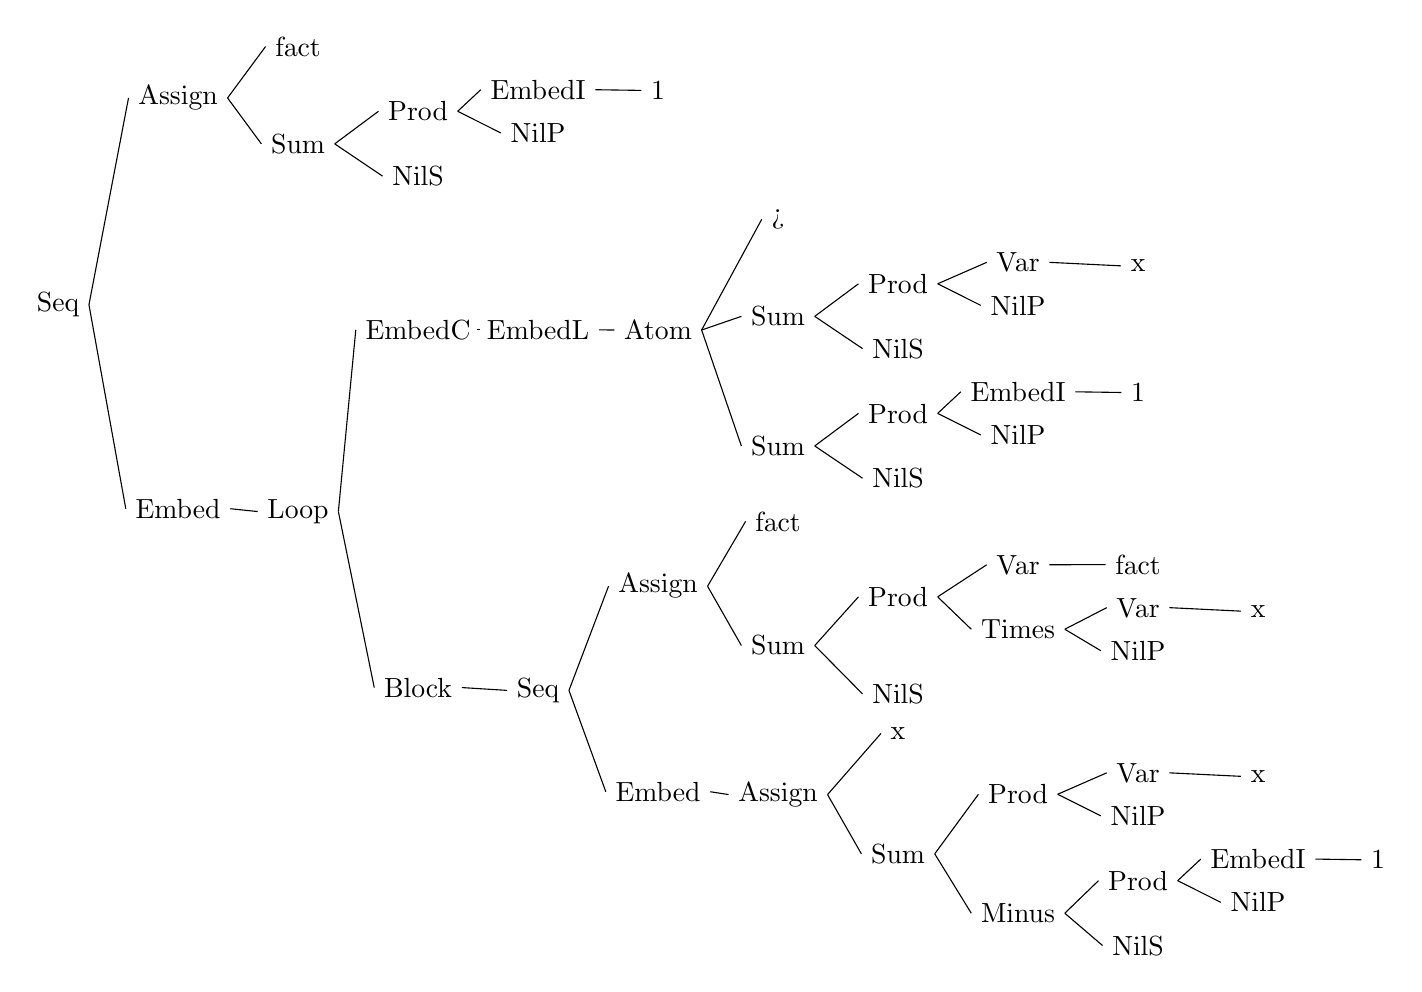
\begin{tikzpicture}[grow'=right, level distance=0.6in]
\Tree [.Seq 
            [.Assign fact 
                          [.Sum 
                                [.Prod 
                                       [.EmbedI 1 ] 
                                       NilP ]
                                NilS ]]
            [.Embed 
                    [.Loop
                           [.EmbedC 
                                    [.EmbedL 
                                             [.Atom > 
                                                    [.Sum 
                                                          [.Prod 
                                                                 [.Var x ]
                                                                 [.NilP ]]
                                                          [.NilS ]]
                                                    [.Sum 
                                                          [.Prod 
                                                                 [.EmbedI 1 ]
                                                                 [.NilP ]]
                                                          [.NilS ]]]]]
                    [.Block 
                            [.Seq 
                                  [.Assign
                                           fact 
                                           [.Sum 
                                                 [.Prod 
                                                        [.Var fact ]
                                                        [.Times 
                                                                [.Var x ]
                                                                [.NilP ]]]
                                                 [.NilS ]]]
                                  [.Embed 
                                          [.Assign
                                                   x
                                                   [.Sum 
                                                         [.Prod
                                                                [.Var x ]
                                                                [.NilP ]]
                                                         [.Minus 
                                                                 [.Prod
                                                                        [.EmbedI 1 ]
                                                                        [.NilP ]]
                                                                 [.NilS ]]]]]]]]]]
\end{tikzpicture}

\subsection{Definition derec(G)}
\label{sec-4-6}

\begin{itemize}
\item F"ur alle s $\in$ S $\cup$ BS $\backslash$ Z(G), derec(G)$_{\text{s}}$ = T$_{\Sigma\text{(G'),s}}$
\item F"ur alle s $\in$ S $\backslash$ recs(S) und s $\to$ v $\in$ R und t $\in$ T$_{\Sigma\text{(G'),typ(v)}}$, f$_{\text{s }\to\ \text{v}}^{\text{derec(G)}}$(t) = f$_{\text{s }\to\ \text{v}}$(t)
\item F"ur alle s $\to$ v $\in$ nonrecs(R), s $\to$ sw $\in$ R, t $\in$ T$_{\Sigma\text{(G'),typ(v)}}$, t' $\in$ T$_{\Sigma\text{(G'),s'}}$ und u $\in$ T$_{\Sigma\text{(G'), typ(w)}}$ \\ f$_{\text{s }\to\ \text{v}}^{\text{derec(G)}}$(t) = f$_{\text{s }\to\ \text{vs'}}$(t, f$_{\text{s' }\to\ \epsilon}$) \\ f$_{\text{s }\to\ \text{sw}}^{\text{derec(G)}}$(f$_{\text{s }\to\ \text{vs'}}$(t,t'),u) = f$_{\text{s }\to\ \text{vs'}}$(t, f$_{\text{s' }\to\ \text{ws'}}$(u, t'))
\end{itemize}

Mit derec(G) kann man eine Syntaxbaum in G in einen Syntaxbaum der nicht linksrekursiven Grammatik G' umwandeln


\subsection{Wort- und Ableitungsbaumalgebra}
\label{sec-4-7}
Neben T$_{\Sigma\text{(g)}}$ lassen sich auch die Menge der W"orter "uber X und die Menge der Ableitungsb"aume von G zu $\Sigma$(G)-Algebren erweitern.

\subsubsection{Wortalgebra}
\label{sec-4-7-1}
fold$^{\text{Word(G)}}$ bildet Terme auf die entsprechenden W"orter der Sprache. 

\subsubsection{Ableitungsbaumalgebra}
\label{sec-4-7-2}
Bildet auf einen Baum ab, der auch die W"orter darstellt (inklusive der Terminale aus Z(G))

\subsection{Zustandsmodell von JavaLight}
\label{sec-4-8}
\begin{itemize}
\item Sei Store = String $\to$ Z (Variablenbelegung)

\item Wir bilden eine $\Sigma$(JavaLight)-Algebra
\end{itemize}

\subsubsection{Sorten}
\label{sec-4-8-1}
\begin{itemize}
\item A$_{\text{Commands}}$ = A$_{\text{Command}}$ = Store $\to$ Store
\item A$_{\text{Sum}}$ = A$_{\text{Factor}}$ = A$_{\text{Prod}}$ = Store $\to$ Z
\item A$_{\text{Disjunkt}}$ = A$_{\text{Conjunct}}$ = A$_{\text{Literal}}$ = Store $\to$ 2
\end{itemize}

\subsubsection{Operationen}
\label{sec-4-8-2}
F"ur alle f,g: Store $\to$ Store, x $\in$ Store, e: Store $\in$ Z, st $\in$ Store \\ und p: Store $\to$ 2.

\begin{center}
seq$^{\text{A}}$(f, g) = g . f, \\
embed$^{\text{A}}$(f) = block$^{\text{A}}$(f) = f, \\
assign$^{\text{A}}$(x,e)(st) = st[e(st)/x], \\
cond$^{\text{A}}$(p, f, g)(st) = if p(st) then f(st) else g(st), \\
cond1$^{\text{A}}$(p, f)(st) = if p(st) then f(st) else st, \\
loop$^{\text{A}}$(p, f)(st) = if p(st) then loop(p, f)(f(st)) else st. \\
\end{center}

F"ur alle f,g: Store $\to$ Z, x $\in$ String und i $\in$ Z

\begin{center}
sum$^{\text{A}}$(f) = prod$^{\text{A}}$(f) = f, \\
plus$^{\text{A}}$(f, g) = list$^{\text{Store}}$(+)(f, g) = $\lambda$ st. f(st) + g(st), \\
minus$^{\text{A}}$(f, g) = list$^{\text{Store}}$(-)(f, g) = $\lambda$ st. f(st) - g(st), \\
times$^{\text{A}}$(f, g) = list$^{\text{Store}}$(*)(f, g) = $\lambda$ st. f(st) * g(st), \\
div$^{\text{A}}$(f, g) = list$^{\text{Store}}$(/)(f, g) = $\lambda$ st. f(st) / g(st), \\
embedI(i)(st) = i, \\
var(x)(st) = st(x), \\
encloseS$^{\text{A}}$(f) = f.
\end{center}

F"ur alle f, g: Store $\to$ 2, rel $\in$ Rel, e, e': Store $\to$ Z, b $\in$ 2,

\begin{center}
disjunct$^{\text{A}}$(f, g) = lift$^{\text{Store}}$($\lor$)(f,g) = $\lambda$ st. f(st) $\lor$ g(st), \\
conjunct$^{\text{A}}$(f, g) = lift$^{\text{Store}}$($\land$)(f,g) = $\lambda$ st. f(st) $\land$ g(st), \\
atom$^{\text{A}}$(rel, e, e') = lift$^{\text{Store}}$(rel)(e,e') = $\lambda$ st. e(st) rel e'(st), \\
embedC$^{\text{A}}$(f) = embedL$^{\text{A}}$(f) = encloseD$^{\text{A}}$(f) = f, \\
not$^{\text{A}}$(f) = \textlnot{} . f, \\
embedB$^{\text{A}}$(b)(st) = b.
\end{center}

\section{Parser und Compiler f"ur CFGs}
\label{sec-5}

\label{diagram_1}
T$_{\Sigma\text{(G)}}$ \xrightarrow{fold^Z} Z \xrightarrow{evaluate} Mach \\
T$_{\Sigma\text{(G)}}$ \xrightarrow{fold^S} S \xrightarrow{encode} Mach

\begin{itemize}
\item S: Sem, die ebenfalls als $\Sigma$(G)-Algebra gegebene Semantik der Quellsprache L(G)
\item Mach, eine in der Regel unabh"angig von $\Sigma$(G) definiertes Modell der Zielsprache, meist in der Form einer abstrakten Maschine
\item evaluate, ein Interpreter der die Zielsprache in der abstrakten Maschine Mach ausf"uhrt
\item encode, eine Funktion, die Sem auf Mach abbildet und die gew"unschte Arbeitsweise des Compilers auf der semantischen Ebene ausf"uhrt
\end{itemize}

\subsection{Definition Parser}
\label{sec-5-1}

Parser f"ur G: eine S-sortige Funktion
\begin{center}
parse$_{\text{G}}$: X$^{\text{*}}$ $\to$ M(T$_{\Sigma\text{(G)}}$)
\end{center}
die entweder einen Synatxbaum f"ur das Eingabewort erzeugt oder eine Fehlermeldung zur"uck gibt. (Syntaxbaum und Fehlermeldung sind abh"anig von der Monade M)

\subsection{Funktoren und Monaden}
\label{sec-5-2}

\subsubsection{Definition Kategorie}
\label{sec-5-2-1}
Eine Kategorie K besteht aus
\begin{itemize}
\item einer - ebenfalls mit K bezeichneten- Klasse von K-Objekten
\item f"ur alle A.B $\in$ K einer Menge K(A,B) von K-Morphismen
\item einer assoziativen Komposition
\end{itemize}
\begin{center}
. : K(A,B) \texttimes{} K(B, C) $\to$ K(A,C) 
\\ (f,g) $\to$ g . f 
\end{center}
\begin{itemize}
\item einer Identit"at id$_{\text{A}}$ $\in$ K(A,A), die bez"uglich . neutral ist
\end{itemize}

\subsubsection{Defintion Funktor}
\label{sec-5-2-2}
Seien K und L Kategorien. Ein Funktor F: K $\to$ L ist eine Funktion(m"ussen das wirklich Funktionen sein?), die jedem K-Objekt ein L-Objekt und jedem 
K-Morphismus f: A $\to$ B eine L-Morphismus F(f): F(A) $\to$ F(B)  zuordnet, sowie folgende Gleichungen erf"ullt:
\begin{itemize}
\item F"ur alle K-Objekte A, F(id$_{\text{A}}$) = id$_{\text{F(A)}}$
\item F"ur alle K-Morphismen f: A $\to$ B und g: B $\to$ C, F(g . f) = F(g) . F(f)
\item Funktoren lassen sich wie Funktionen zu neuen Funktoren komponieren.
\end{itemize}

\begin{enumerate}
\item Beispiele
\label{sec-5-2-2-1}
\begin{itemize}
\item Sei B $\in$ L. Der konstante Funktor const(B): K $\to$ L ordnet jedem K-Objekt B und jedem K-Morphismus die Identit"at auf B zu
\item Der Diagonalfunktor $\Delta$$_{\text{K}}$: K $\to$ K$^{\text{2}}$ ordnet jedem K-Objekt A das Paar (A,A) und jedem K-Morphismus f das Paar (f,f) zu
\item Produktfunktor, \_ \texttimes{} \_ : Set$^{\text{2}}$ $\to$ Set ordnet jedem Mengenpaar (A,B) die Menge A \texttimes{} B und jedem Funktionspaar (f: A $\to$ B, g: C $\to$ D) die Funktion f \texttimes{} g =$_{\text{def}}$ $\lambda$(a,c).(f(a),g(c)) zu
\item Ausnahmefunktor \_ + E : Set $\to$ Set ordnet jeder Menge A die Menge A + E zu und jeder Funktion f: A $\to$ B die Funktion
\end{itemize}
\begin{center}
f + E: A + E $\to$ B + E \\
(a, 1) $\to$ (f(a), 1) \\
(e, 2) $\to$ (e, 2) \\
\end{center}
\end{enumerate}

\subsubsection{Definition Nat"urliche Transformation}
\label{sec-5-2-3}
Seien F, G: K $\to$ L Funktoren. Eine nat"urliche Transformation $\tau$: F $\to$ G ordnet jedem K-Objekt A einen L-Morphismus $\tau$$_{\text{A}}$: F(A) 
$\to$ G(A) derart, dass f"ur alle K-Morphismen f:A $\to$ B das gilt:

\begin{itemize}
\item F(A) $\to$$^{\tau_{\text{A}}}$ G(A)
\item F(A) $\to$$^{\text{F(f)}}$ F(B)
\item F(B) $\to$$^{\tau_{\text{B}}}$ G(B)
\item G(A) $\to$$^{\text{G(f)}}$ G(B)
\end{itemize}

\subsubsection{Definition Monade}
\label{sec-5-2-4}
Ein Funktor M: K $\to$ K hei"st Monade, wenn es zwei nat"urliche Transformationen $\eta$: Id$_{\text{K}}$ $\to$ M (Einheit) und $\mu$: M . M $\to$ M 
(Multiplikation) gibt, die f"ur alle A $\in$ K folgednes gelten lassen:

\begin{itemize}
\item Seite 154 Folienscript
\end{itemize}

\begin{enumerate}
\item Beispiel Ausnahmefunktor
\label{sec-5-2-4-1}

\begin{itemize}
\item $\eta$$_{\text{A}}$: A $\to$ A + E \\ $\eta$$_{\text{A}}$(a) = (a,1)
\item $\mu$$_{\text{A}}$: (A + E) + E \\ $\mu$$_{\text{A}}$( ((a,1),1) ) = (a,1) \\ $\mu$$_{\text{A}}$( ((e,2),1) ) = (e,2) \\ $\mu$$_{\text{A}}$( (e,2) ) = (e,2)
\end{itemize}

\item Der bind-Operator
\label{sec-5-2-4-2}
Seien A und B Mengen

\begin{center}
>>=: M(A) \texttimes{} (A $\to$ M(B)) $\to$ M(B) \\
(>>= f) = $\mu$$_{\text{B}}$ . M(f)
\end{center}

\item Intuitive Erkl"arung einer Monade
\label{sec-5-2-4-3}

Intuitiv stellt man sich ein monadisches Object m $\in$ M(A) als Berechnung vor, die eine -evt leere- Menge von Werten in A erzeugt. 
Ein Ausdruck der Form \emph{>>= f} wird dann wie folgt ausgewertet: Die von m berechneten Werte a $\in$ A werden als Eingabe an die Berechnung
von f "ubergeben und von f(a) verarbeitet.

\item Es ergeben sich ein paar Eigenschaften
\label{sec-5-2-4-4}
\begin{itemize}
\item m >>= $\eta$$_{\text{A}}$ = m
\item $\eta$$_{\text{A}}$(a) >>= f = f(a)
\item (m >>= f) >>= g = m >>= $\lambda$ a. f(a) >>= g
\item M(h)(m) = m >>= $\mu$$_{\text{B}}$ . h
\item $\eta$$_{\text{A}}$(m') = m' >>= id$_{\text{M}}$(A)
\end{itemize}

\item Plusmonade
\label{sec-5-2-4-5}
Plusmonaden haben zus"atzlich eine parallele \textbf{Komposition}
\begin{center}
$\oplus$: M \texttimes{} M =$_{\text{def}}$ \_ \texttimes{} \_ . $\Delta$ . M $\to$ M
\end{center}
\end{enumerate}

\subsubsection{Compilermonade}
\label{sec-5-2-5}
Sei M: Set$^{\text{S}}$ $\to$ Set$^{\text{S}}$ eine Monade mit der Einheit $\eta$, bind-Operator >>= und paralleler Komposition $\oplus$, set: M $\to$ P eine 
weitere nat"urliche Transformation und 
\begin{center}
E = \{m $\in$ M(A) | set$_{\text{A}}$(m) = $\emptyset$, A $\in$ Set$^{\text{S}}$\}
\end{center}
"Menge der Ausnahmewerte" \\

M hei"st Compilermonade, wenn f"ur alle Mengen A und B, m, m', m'' $\in$ M(A), e $\in$ E, f: A $\to$ M(B), h: A $\to$ B und a $\in$ A Folgendes gilt:
\begin{center}
(m $\oplus$ m') $\oplus$ m'' = m $\oplus$ (m' $\oplus$ m'') \\
M(h)(e) = e \\
M(h)(m $\oplus$ m') = M(h)(m) $\oplus$ M(h)(m') \\
set$_{\text{A}}$(m $\oplus$ m') = set$_{\text{A}}$(m) $\cup$ set$_{\text{A}}$(m') \\
set$_{\text{A}}$($\eta$$_{\text{A}}$(a)) = \{a\} \\
set$_{\text{B}}$(m >>= f) = $\cup$\{set$_{\text{B}}$(f(a)) | a $\in$ set$_{\text{A}}$(m)\}
\end{center}

\subsubsection{Monadenbasierte Parser und Compiler}
\label{sec-5-2-6}

\begin{itemize}
\item Sei G = (S, BS, R) LL-kompilierbar
\item G' die daraus gebildete nicht-linksrekursive Grammatik
\item X = $\cup$ BS
\item $\Sigma$(G) = (S, F)
\item M : Set$^{\text{S}}$ $\to$ Set$^{\text{S}}$
\end{itemize}

Ein Compiler f"ur G in die als $\Sigma$(G)-Algebra A formulierte Zielsprache einen Parser f"ur G mit der Faltung in A der vom Parser 
erzeugten Syntaxbaume komponieren.
Daher passen wir die "Ubersetzungsfunktion ein bisschen an:

\label{compile_funktion}
\begin{center}
compile$_{\text{G}}^{\text{A}}$ = X$^{\text{*}}$ $\to$$^{\text{compile}_{\text{G}}^{\text{T}_{\Sigma\text{(G)}}}}$ M(T$_{\Sigma\text{(G)}}$) $\to$$^{\text{M(fold}_{\text{A}}\text{)}}$ M(A)
\end{center}

Ist G linksrekursiv terminiert das evt nicht, daher fordern wir in dem Fall:

\begin{center}
compile$_{\text{G}}^{\text{A}}$ = X$^{\text{*}}$ $\to$$^{\text{parse}_{\text{G}}^{\text{T}_{\Sigma\text{(G)}}}}$ M(T$_{\Sigma\text{(G')}}$) $\to$$^{\text{M(fold}_{\text{derec(A))}}}$ M(A)
\end{center}

Es gilt die Vertr"aglichkeit mit $\Sigma$-Homomorphismen (eingebettet in die Monade nat"urlich)

Gilt \ref{compile_funktion}, dann folgt aus \ref{diagram_1}: 
\begin{itemize}
\item X$^{\text{*}}$ $\to$$^{\text{compile}_{\text{G}}^{\text{A}}}$ M(A) $\to$$^{\text{M(evaluate)}}$ M(Mach) \\
\item X$^{\text{*}}$ $\to$$^{\text{compile}_{\text{G}}^{\text{S}}}$ M(S) $\to$$^{\text{M(encode)}}$ M(Mach)
\end{itemize}


\section{LL Kompiler}
\label{sec-6}

Das erste L steht f"ur die Verarbeitung von \textbf{Links} nach Rechts. Das zweite L steht f"ur das bilden einer \textbf{Linksableitung}.

\begin{itemize}
\item G = (S, BS, R)
\item G' = (S', BS, R')
\item X = $\cup$ BS
\item M eine Compilermonade
\item errmsg: X$^{\text{*}}$ $\to$ E
\item A = (A, Op) eine $\Sigma$(G)-Algebra
\item \emph{compile$_{\text{G}}$} hei"st LL-Compiler, wenn (compile$^{\text{A}}_{\text{G,s}}$: X$^{\text{*}}$ $\to$ M(A$_{\text{s}}$))$_{\text{s} \in \text{S}}$
\item compile$_{\text{G,s}}^{\text{A}}$(w) = trans$_{\text{s}}^{\text{A}}$(w) >>= $\lambda$(a, w). if w = $\epsilon$ then $\eta$$_{\text{A}}$(a) else errmsg(w), wobei f"ur alle s $\in$ S' $\cup$ BS \\ trans$_{\text{s}}^{\text{A}}$ : X$^{\text{*}}$ $\to$ M(A$_{\text{s}}$ \texttimes{} X$^{\text{*}}$) wie folgt definiert ist:
\end{itemize}

\subsection{Fall 1: s $\in$ BS. F"ur alle x $\in$ X und w $\in$ X$^{\text{*}}$}
\label{sec-6-1}

\begin{center}
trans$_{\text{s}}^{\text{A}}$(xw) = if x $\in$ s then $\eta$$_{\text{A }\texttimes{}\ \text{X}^{\text{*}}}$(x,w) else errmsg(xw) \\
trans$_{\text{s}}^{\text{A}}$($\epsilon$) = errmsg($\epsilon$)
\end{center}

\subsection{Fall 2: s $\in$ S'. F"ur alle w $\in$ X$^{\text{*}}$,}
\label{sec-6-2}

\begin{center}
trans$_{\text{s}}^{\text{A}}$(w) = $\oplus$$_{\text{r=(s }\to\ \text{e)}\in\ \text{R}}$ try$_{\text{r}}^{\text{A}}$(w)
\end{center}


F"ur alle r = (s $\to$ (e$_{\text{1}}$,..,e$_{\text{n}}$))$\in$ R' und w $\in$ X$^{\text{*}}$,
\begin{center}
try$_{\text{r}}^{\text{A}}$(w) = trans$_{\text{e}_{\text{1}}}^{\text{A}}$ >>= $\lambda$(a$_{\text{1}}$,w$_{\text{1}}$). \ldots{}\ldots{} trans$_{\text{e}_{\text{n}}}^{\text{A}}$(w$_{\text{n-1}}$) >>= $\lambda$(a$_{\text{n}}$, w$_{\text{n}}$).$\eta$$_{\text{A }\texttimes{}\ \text{X}^{\text{*}}}$(f$_{\text{r}}^{\text{derec(A)}}$(a$_{\text{i}_{\text{1}}}$,..,a$_{\text{i}_{\text{k}}}$),w$_{\text{n}}$)
\end{center}
wobei \{i$_{\text{1}}$,..,i$_{\text{k}}$\} = \{1 $\le$ i $\le$ n | e$_{\text{i}}$ $\in$ S' $\cup$ BS $\backslash$ Z(G)\} \\


\textbf{\uline{Ein Beispiel ist auf Seite 170 im Folienscript. Das JavaLight+ Beispiel beginnt auf Seite 172}} 

\section{LR Kompiler}
\label{sec-7}

\begin{itemize}
\item Konstruieren \textbf{Rechtsreduktion} ($\Rightarrow$ Rechtsableitung)
\item Entspricht dem \emph{mit dem Bl"attern beginnender Aufbau eines Syntaxbaumes}, daher \textbf{Bottom-up} Compiler
\item LR-Compiler sind auf LR(\emph{k})-Grammatiken beschr"ankt
\item Sei G = (S, BS, R) eine CFG und X = $\cup$ BS
\item Vorraussetzung: \emph{start} $\in$ S und \emph{start} kommt in keiner Regel auf der rechten Seite vor
\end{itemize}

\subsection{LR(k) Grammatiken}
\label{sec-7-1}
Eine Grammatik ist eine LR(k) Grammatik, wenn das vorrauslesen von k Symbolen reicht, damit man entscheiden kann ob ein weiteres 
Zeichen gelesen werden muss oder eine Reduktion durchgef"uhrt werden muss (und wenn ja welche). Au"serdem m"ussen die BS disjunkt sein.

\subsubsection{Definition first- und follow- Wormengen}
\label{sec-7-1-1}
Sei k > 0, $\alpha$ $\in$ (S $\cup$ BS)$^{\text{*}}$ und s $\in$ S
\begin{center}
first$_{\text{k}}$($\alpha$) = \{$\beta$ $\in$ BS$^{\text{k}}$ | $\exists$ $\gamma$ $\in$ BS$^{\text{*}}$: $\alpha$ $\to$$^{\text{*}}_{\text{G}}$ $\beta$$\gamma$\} $\cup$ \{$\beta$ $\in$ BS$^{\text{<k}}$ | $\alpha$ $\to$$^{\text{*}}_{\text{G}}$ $\beta$\}
follow$_{\text{k}}$(s) = \{$\beta$ $\in$ BS$^{\text{k}}$ | $\exists$ $\alpha$, $\gamma$ $\in$ BS$^{\text{*}}$: start $\to$$^{\text{*}}_{\text{G}}$ $\alpha$ s $\beta$$\gamma$\} $\cup$ \{$\alpha$ $\in$ BS$^{\text{<k}}$ | start $\to$$^{\text{*}}_{\text{G}}$ $\alpha$ s $\beta$\}
first($\alpha$) = first$_{\text{1}}$($\alpha$)
follow(s) = follow$_{\text{1}}$(s)
\end{center}

Sei recog$_{\text{1}}$ ein Erkenner f"ur die Sprache (Definition auf Seite 190)

\subsection{LR-Automat}
\label{sec-7-2}
Zustandsmenge:
\begin{itemize}
\item Q$_{\text{G}}$ = \{state($\phi$) | $\phi$ $\in$ (S $\cup$ BS)$^{\text{*}}$\}
\end{itemize}

\emph{partielle} Transitionsfunktion (auch goto-Tabelle genannt) 
\begin{itemize}
\item $\delta$: Q$_{\text{G}}$ $\to$ Q$_{\text{G}}^{\text{S }\cup\ \text{BS}}$ \\ state($\phi$) = $\lambda$(s).state($\phi$ s)
\end{itemize}

\subsubsection{Simultane induktive Definition von Q$_{\text{G}}$ und $\delta$$_{\text{G}}$}
\label{sec-7-2-1}
\begin{center}
start $\to$ $\alpha$ $\in$ R $\Rightarrow$ (start, $\epsilon$, $\alpha$, $\epsilon$) $\in$ q$_{\text{0}}$ \\
(s, $\alpha$, s', $\beta$, u) $\in$ q $\land$ s' $\to$ $\gamma$ $\in$ R $\land$ v $\in$ first($\beta$ u) $\Rightarrow$ (s', $\epsilon$, $\gamma$, v) $\in$ q \\
(s, $\alpha$, s'$\beta$, u) $\in$ q, s' $\in$ S $\cup$ BS $\Rightarrow$ (s, $\alpha$ s', $\beta$, u) $\in$ $\delta$$_{\text{G}}$(q)(s')
\end{center}

\begin{itemize}
\item h: (S $\cup$ BS)$^{\text{*}}$ $\to$ Q$^{\text{*}}_{\text{G}}$
\item state($\epsilon$) =$_{\text{def}}$ $\lambda$($\epsilon$). q$_{\text{0}}$
\item $\lambda$(s$_{\text{1}}$,..,s$_{\text{n}}$). (state(s$_{\text{1}}$\ldots{}s$_{\text{n}}$), state(s$_{\text{1}}$\ldots{}s$_{\text{n-1}}$),.., state(s$_{\text{1}}$), state($\epsilon$))
\end{itemize}


Wir definieren recog$_{\text{2}}$: Q$^{\text{*}}_{\text{G}}$ $\to$ 2$^{\text{X}^{\text{*}}}$ \\
F"ur alle q, q$_{\text{i}}$ $\in$ Q$_{\text{G}}$, qs $\in$ Q$^{\text{*}}_{\text{G}}$, x $\in$ X und w $\in$ X$^{\text{*}}$,
\begin{itemize}
\item recog$_{\text{2}}$(q:qs)(xw) = recog$_{\text{2}}$($\delta$$_{\text{G}}$(q)(x):q:qs)(w) \\ falls $\exists$ (s, $\alpha$, $\beta$, $\epsilon$) $\in$ q : $\beta$ $\neq$ $\epsilon$, x $\in$ first($\beta$) $\cap$ Z(G)
\item recog$_{\text{2}}$(q:qs)(xw) = recog$_{\text{2}}$($\delta$$_{\text{G}}$(q)(B):q:qs)(w) \\ falls $\exists$ (s, $\alpha$, $\beta$, $\epsilon$) $\in$ q, B $\in$ BS: \\ $\beta$ $\neq$ $\epsilon$, x $\in$ B $\in$ first($\beta$)
\item recog$_{\text{2}}$(q$_{\text{1}}$: \ldots{} :q$_{\text{|}\alpha\text{|}}$:q:qs)(w) = recog$_{\text{2}}$($\delta$$_{\text{G}}$(q)(s):q:qs)(w) \\ falls $\exists$ (s, $\alpha$, $\epsilon$ u) $\in$ q$_{\text{1}}$:s $\neq$ start, \\ w = $\epsilon$ = u $\lor$ head(w) = u $\in$ Z(G) $\lor$ \\ head(w) $\in$ u $\in$ BS
\item recog$_{\text{2}}$(q:qs)($\epsilon$) = 1 falls $\exists$ $\varphi$ : (start, $\varphi$, $\epsilon$, $\epsilon$) $\in$ q
\item recog$_{\text{2}}$(qs)(w) = 0 sonst
\end{itemize}

Offenbar gilt recog$_{\text{1}}$ = recog$_{\text{2}}$ \bigcirc h.

Zur optimieren verwenden wir eine Aktionstabelle 
\begin{itemize}
\item act$_{\text{G}}$: Q$_{\text{G}}$ \texttimes{} (BS $\cup$ 1) $\to$ R $\cup$ \{shift, error\}
\end{itemize}
F"ur alle u $\in$ BS $\cup$,

\begin{itemize}
\item act$_{\text{G}}$(q, u) = shift falls $\exists$ (s, $\alpha$, $\beta$, $\epsilon$) $\in$ q: $\beta$ $\neq$ $\epsilon$, u $\in$ first($\beta$), \\ s $\to$ $\alpha$ falls $\exists$ (s, $\alpha$, $\epsilon$ u) $\in$ q, \\ \emph{error} sonst
\end{itemize}

Dann erh"alt man eine Kompaktedefinition f"ur recog$_{\text{2}}$:

F"ur alle q, q$_{\text{i}}$ $\in$ Q$_{\text{G}}$, qs $\in$ Q$^{\text{*}}_{\text{G}}$, x $\in$ X und w $\in$ X$^{\text{*}}$,
\begin{itemize}
\item recog$_{\text{2}}$(q:qs)(xw) = recog$_{\text{2}}$($\delta$$_{\text{G}}$(q)(x):q:qs)(w) \\ falls x $\in$ Z(G), act$_{\text{G}}$(q, x) = shift
\item recog$_{\text{2}}$(q:qs)(xw) = recog$_{\text{2}}$($\delta$$_{\text{G}}$(q)(B):q:qs)(w) \\ falls $\exists$ B $\in$ BS : x $\in$ B, act$_{\text{G}}$(q, B) = shift
\item recog$_{\text{2}}$(q$_{\text{1}}$:\ldots{}:q$_{\text{|}\alpha\text{|}}$:q:qs)(w) = recog$_{\text{2}}$($\delta$$_{\text{G}}$(q)(s):q:qs)(w) \\ falls $\exists$ u $\in$ BS $\cup$ 1: act$_{\text{G}}$(q$_{\text{1}}$, u) = s $\to$ $\alpha$,\\ w = $\epsilon$ = u $\lor$ head(w) = u $\in$ Z(G) $\lor$ \\ head(w) $\in$ u $\in$ BS
\item recog$_{\text{2}}$(q:qs)($\epsilon$) = 1 falls act$_{\text{G}}$(q, $\epsilon$) = start $\to$ $\alpha$
\item recog$_{\text{2}}$(qs)(w) = 0 sonst
\end{itemize}

Beispiel f"ur SAB2 auf Seite 197 im Skript.

\subsubsection{Formulierung der Korrektheit von compile$_{\text{G}}$}
\label{sec-7-2-2}
\begin{itemize}
\item F"ur alle w $\in$ X$^{\text{*}}$ und t $\in$ T$_{\Sigma\text{(G), start}}$, \\ compile$_{\text{G}}^{\text{A}}$(q$_{\text{0}}$, $\epsilon$)(w) = $\eta$(fold$^{\text{A}}$(t)) $\Rightarrow$ fold$^{\text{Word(G)}}$(t) = w, \\ compile$_{\text{G}}^{\text{A}}$(q$_{\text{0}}$, $\epsilon$)(w) = error(w) $\Rightarrow$ w $\notin$ L(G)$_{\text{start}}$
\end{itemize}
\subsubsection{Beispiel SAB2; Seite 203}
\label{sec-7-2-3}

\subsubsection{Beispiel yacc; Seite 204}
\label{sec-7-2-4}

\subsubsection{Sprachklassen-Hierarchie}
\label{sec-7-2-5}

\begin{itemize}
\item CFG $\subset$ LR(k) $\subset$ LL(k)
\item LR(k) $\subset$ LALR(k) $\subset$ SLR(k)
\item LL(k)-Grammatiken sind \uline{kurz gesagt} diejenigen nicht-linksrekursiven CFGs, deren LL-Parser ohne Backtracking auskommen.
\item F"ur jeden Grammatiktyp T bedeutet die Formulierung \textbf{L ist eine T-Sprache} lediglich, dass eine T-Grammatik \emph{existiert} die L erzeugt
\end{itemize}

\begin{enumerate}
\item Kommentar zu LL-Compiler
\label{sec-7-2-5-1}

W"ahrend der LL-Compiler von Kapitel 6 - nach Beseitigung von Linksrekursion - jede kontexfreie Grammatik verarbeitet, selbst dann,
wenn sie mehrdeutig ist, zeigt die obige Grafikm dass die Forderung, dabei ohne Backtracking auszukommen, die Klasse der kompilierbaren 
Sprache erheblich einschr"ankt: Unter dieser Bedingung ist die bottom-up "Ubersetzung offenbar m"achtiger als die top-down Compilation.

Umgekehrt w"are es den Versuch wert (z.B. in Form einer BA), in Anlehnung an den obigen Compiler f"ur LR(1)-Grammatiken einen bottom-up
Compiler mit Backtracking zu entwickeln. Da die Determinismusforderung wegfiele, br"auchten wir keinen Lookahead beim Verarbeiten der 
Eingabe, womit die Zust"ande generell nur aus Tripeln best"unden - wie im beispiel Yacc.
\end{enumerate}

\section{Haskell: Typen und Funktionen}
\label{sec-8}
Ich hoffe ihr seid fit in Haskell

\section{Haskell: Listen}
\label{sec-9}

\section{Haskell: Datentypen und Typklassen}
\label{sec-10}

\section{Algebren in Haskell}
\label{sec-11}

Sei $\Sigma$ = (S, F) eine Signatur, obs($\Sigma$) = \{x$_{\text{1}}$,\ldots{},x$_{\text{k}}$\}, S = \{s$_{\text{1}}$,\ldots{},s$_{\text{m}}$\} und F = \{f$_{\text{1}}$: e$_{\text{1}}$ $\to$ e'$_{\text{1}}$ .. f$_{\text{n}}$: e$_{\text{n}}$ $\to$ e'$_{\text{n}}$\}.\\
Jede $\Sigma$-Algebra entspricht einem Element des folgenden polymorphen Datentyps:
\begin{verbatim}
data Sigma x1 ... xk s1 ... sm = Sigma {f1 :: e1 -> e1', ...,
					fn :: en -> en'}
\end{verbatim}

Die Sorten und Operationen von $\Sigma$ werden durch Typvariablen bzw. Destruktoren wiedergegeben und durch die Tr"agermengen bzw. 
kaskadierten Funktionen der jeweiligen Algebra instanziiert.

Um eine Signatur $\Sigma$ in Haskell zu implementieren, gen"ugt es daher, den Datentyp ihrer Algebren nach obigem Schema zu formulieren.

Der Datentyp Sigma(x$_{\text{1}}$)\ldots{}(x$_{\text{k}}$) repr"asentieren die Tr"agermengen einzelner Algebren.

\subsection{Beispiel f"ur Nat}
\label{sec-11-1}

\begin{verbatim}
--natT implementiert T_Nat
data Nat nat = Nat {zero :: nat, succ :: nat -> nat}

natT :: Nat Int
natT = Nat {zero = 0, succ = (+1)}

--listT implementiert T_list(X)
data List x list = List {nil :: list, cons :: x -> list -> list}

listT :: List x [x]
listT = List {nil = [], cons = (:)}

--Beispiel foldList

foldList :: List x list -> [x] -> list
foldList alg [] = nil alg
foldList alg (x:s) = cons alg x $ foldList alg s
\end{verbatim}

Weitere Beispiele ab Seite 252.

\subsection{Datentypen der JavaLight-Algebren}
\label{sec-11-2}

\begin{verbatim}
data JavaLight commands command sum prod factor disjunct conjunct literal =
  JavaLight {seq_ :: command -> commands -> commands
	    ,embed :: command -> commands
	    ,block :: commands -> command
	    ,assign :: String -> sum -> command
	    ,cond :: disjunct -> command -> command -> command
	    ,cond1, loop :: disjunct -> command -> command
	    ,sum_ :: prod -> sum
	    ,plus, minus :: sum -> prod -> sum
	    ,prod :: factor -> prod
	    ,times, div_ :: prod -> factor -> prod
	    ,embedI :: Int -> factor
	    ,var :: String -> factor
	    ,encloseS :: sum -> factor
	    ,disjunct :: conjunct -> disjunct -> disjunct
	    ,embedC :: conjunct -> disjunct
	    ,conjunct :: literal -> conjunct -> conjunct
	    ,embedL :: literal -> conjunct
	    ,not_ :: literal -> literal
	    ,atom :: String -> sum -> sum -> literal
	    ,embedB :: Bool -> literal
	    ,encloseD :: disjunct -> literal}

data SumProd sum sumsect prod prodsect factor =
  SumProd {sum' :: prod -> sumsect -> sum
	  ,plus', minus' :: prod -> sumsect -> sumsect
	  ,nilS :: sumsect
	  ,prod' :: factor -> prodsect -> prod
	  ,times', div' :: factor -> prodsect -> prodsect
	  ,nilP :: prodsect}

derec :: JavaLight s1 s2 sum prod factor s3 s4 s5 -> SumProd sum (sum -> sum) prod (prod -> prod) factor
derec alg = SumProd {sum' = \a g -> g $ sum_ alg a,
		     plus' = \a g x -> g $ plus alg x a,
		     minus' = \a g x -> g $ minus alg x a,
		     nilS = id,
		     prod' = \a g -> g $ prod alg a,
		     times' = \a g x -> g $ times alg x a,
		     div' = \a g x -> g $ div_ alg x a,
		     nilP = id}
\end{verbatim}


\subsection{Die Termalgebra von JavaLight}
\label{sec-11-3}

\begin{verbatim}
data Commands = Seq (Command, Commands) | Embed Command deriving Show

data Command = Block Commands | Assign (String, Sum) |
	       Cond (Disjunct, Command, Command) | Cond1 (Disjunct, Command) |
	       Loop (Disjunct, Command) deriving Show

data Sum = SUM Prod | PLUS (Sum, Prod) | MINUS (Sum, Prod) deriving Show

data Prod = PROD Factor | TIMES (Prod, Factor) | DIV (Prod, Factor) deriving Show

data Factor = EmbedI Int | Var String | EncloseS Sum deriving Show

data Disjunct = Disjunct (Conjunct, Disjunct) | EmbedC Conjunct deriving Show

data Conjunct = Conjunct (Literal, Conjunct) | EmbedL Literal deriving Show

data Literal = Not Literal | Atom (String, Sum, Sum) | EmbedB Bool | EncloseD Disjunct deriving Show


javaTerm :: JavaLight Commands Command Sum Prod Factor Disjunct Conjunct Literal
javaTerm = JavaLight { seq_ = curry Seq, embed = Embed, block = Block
		     ,assign = curry Assign, cond = curry3 Cond, cond1 = curry Cond1
		     ,loop = curry Loop, sum_ = SUM, plus = curry PLUS
		     ,minus = curry MINUS, prod = PROD, times = curry TIMES
		     ,div_ = curry DIV, embedI = EmbedI, var = Var
		     ,encloseS = EncloseS, disjunct = curry Disjunct, embedC = EmbedC
		     ,conjunct = curry Conjunct, embedL = EmbedL, not_ = Not
		     ,atom = curry3 Atom, embedB = EmbedB, encloseD = EncloseD}

javaWord :: JavaLight String String String String String String String
javaWord = JavaLight {seq_ = (++)
		     ,embed = id
		     ,block = \cs -> " {" ++ cs ++ "}"
		     ,assign = \x e -> x ++ " = " ++ e ++ "; "
		     ,cond = \e c c' -> "if " ++ e ++ c ++ " else" ++ c'
		     ,cond1 = \e c -> "if " ++ e ++ c
		     ,loop = \e c -> "while " ++ e ++ c
		     ,sum_ = id
		     ,plus = \e e' -> e ++ '+':e'
		     ,minus = \e e' -> e ++ '-':e'
		     ,prod = id
		     ,times = \e e' -> e ++ '*':e'
		     ,div_ = \e e' -> e ++ '/':e'
		     ,embedI = show
		     ,var = id
		     ,encloseS = \e -> '(' : e ++ ")"
		     ,disjunct = \e e' -> e ++ " || " ++ e'
		     ,embedC = id
		     ,conjunct = \e e' -> e ++ " && " ++ e'
		     ,embedL = id
		     ,not_ = \be -> '!' : be
		     ,atom = \rel e e' -> e ++ rel ++ e'
		     ,embedB = show
		     ,encloseD = \e -> '(' : e ++ ")"}
\end{verbatim}

\subsection{Zustandsmodell von JavaLight}
\label{sec-11-4}

\begin{verbatim}
type St a = Store -> a

rel :: String -> Int -> Int -> Bool
rel = \case "<" -> (<)
	    ">" -> (>)
	    "<=" -> (<=)
	    ">=" -> (>=)
	    "==" -> (==)
	    "!=" -> (/=)

javaState :: JavaLight (St Store) (St Store) (St Int) (St Int) (St Int) (St Bool) (St Bool) (St Bool)
javaState = JavaLight {seq_ = flip (.)
		      ,embed = id
		      ,block = id
		      ,assign = \x e st -> update st x $ e st
		      ,cond = cond
		      ,cond1 = \p f -> cond p f id
		      ,loop = loop
		      ,sum_ = id
		      ,plus = liftM2 (+)
		      ,minus = liftM2 (-)
		      ,prod = id
		      ,times = liftM2 (*)
		      ,div_ = liftM2 div
		      ,embedI = const
		      ,var = flip ($)
		      ,encloseS = id
		      ,disjunct = liftM2 (||)
		      ,embedC = id
		      ,conjunct = liftM2 (&&)
		      ,embedL = id
		      ,not_ = (not .)
		      ,atom = liftM2 . rel
		      ,embedB = const
		      ,encloseD = id}
	    where
	      cond :: St Bool -> St Store -> St Store -> St Store
	      cond p f g st = if p st then f st else g st
	      loop :: St Bool -> St Store -> St Store
	      loop p f st = if p st then loop f $ f st else st
\end{verbatim}

\subsubsection{Interpretation eines JavaLight Programms}
\label{sec-11-4-1}

prog = fact = 1; while x > 1 \{fact = fact*x; x = x-1;\}

compile$^{\text{A}}_{\text{JavaLight}}$(prog) : Store $\to$ Store \\
compile$^{\text{A}}_{\text{JavaLight}}$ = $\lambda$(store). $\lambda$(z). if z = x then 0 else if z = fact then store(x)! else store(z)

\subsection{Ableitungsbaumalgebra von JavaLight}
\label{sec-11-5}

\begin{verbatim}
type TS = Tree String

javaDeri :: JavaLight TS TS TS TS TS TS TS
javaDeri = JavaLight {seq_ = \c c' -> F "Commands" [c,c']
		     ,embed = \c -> F "Commands" [c]
		     ,assign = \x e -> command [leaf x, leaf "=", e, leaf ";"]
		     ,cond = \e c c' -> command [leaf "if", e, c, leaf "else", c']
		     ,cond1 = \e c -> command [leaf "if", e, c]
		     ,loop = \e c -> command [leaf "while", e, c]
		     ,sum_ = \e -> F "Sum" [e]
		     ,plus = \e e' -> F "Sum" [e, e']
		     ,minus = \e e' -> F "Sum" [e, e']
		     ,prod = \e -> F "Prod" [e]
		     ,times = \e e' -> F "Prod" [e, e']
		     ,div_ = \e e' -> F "Prod" [e, e']
		     ,embedI = \i -> factor [leaf $ show i]
		     ,var = \x -> factor [leaf x]
		     ,encloseS = \e -> factor [leaf "(", e, leaf ")"]
		     ,disjunct = \e e -> F "Disjunct" [e, leaf, "||", e']
		     ,embedC = \e -> F "Disjunct" [e]
		     ,conjunct = \e e' -> F "Conjunct" [e, leaf "&&", e']
		     ,embedL = \e -> F "Conjunct" [e]
		     ,not_ = \be -> literal [leaf "!", be]
		     ,atom = \rel e e' -> literal [e, leaf rel, e']
		     ,embedB = \b -> literal [leaf $ show b]
		     ,encloseD = \e -> literal [leaf "(", e, leaf ")"]}
	   where
	     command = F "Command"
	     factor = F "Factor"
	     literal = F "Literal"
	     leaf = flip F []
\end{verbatim}

\subsection{Beispiel XMLstore-Algebren (Seite 265)}
\label{sec-11-6}

\section{Attributierte "Ubersetzung}
\label{sec-12}
\subsection{Bin"ardarstellung rationaler Zahlen}
\label{sec-12-1}
\subsection{Strings mit Hoch- und Tiefdarstellung}
\label{sec-12-2}
\subsection{"ubersetzung regul"arer Ausdr"uck in erkennenden Automaten}
\label{sec-12-3}
\subsection{Darstellung von Termen als hierarchische Listen}
\label{sec-12-4}
\subsection{Eine kellerbasierte Zielsprache f"ur JavaLight}
\label{sec-12-5}
Der folgende Datentyp liefert die Befehle einer Assemblersprache, die auf einem Keller vom Typ Z und einem Speicher vom Typ
\begin{center}
Store = String $\to$ Z
\end{center}
operiert. Hierbei betrachten wir die Abstraktion eines realen Speichers.

\begin{verbatim}
data StackCom = Push Int | Pop | Load String | Save String | Add |
		Sub | Mul | Div | Or_ | And_ | Inv | Cmp String | Jump Int |
		JumpF Int

type State = ([Int], Store, Int)

executeCom :: StackCom -> State -> State
executeCom com (stack, store, n) =
  case com of Push a -> (a:stack, store, n+1)
	      Pop    -> (tail stack, store, n+1)
	      Load x -> (store x:stack, store, n+1)
	      Save x -> (stack, update store x $ head stack, n+1)
	      Add    -> (a+b:s, store, n+1) where a:b:s = stack
	      Sub    -> (b-a:s, store, n+1) where a:b:s = stack
	      Mul    -> (a*b:s, store, n+1) where a:b:s = stack
	      Div    -> (a`div`b:s, store, n+1) where a:b:s = stack
	      Or_    -> (max a b:s, store, n+1) where a:b:s = stack
	      And_   -> (a*b:s, store, n+1)     where a:b:s = stack
	      Inv    -> ((a+1) `mod`2:s, store, n+1) where a:s = stack
	      Cmp str -> (c:s, store, n+1)
		where a:b:s = stack
		      c = if rel str a b then 1 else 0
	      Jump k  -> (stack, store, k)
	      JumpF k -> (stack, store, if a == 0 then k else n+1) where a:_ = stack

execute :: [StackCom] -> State -> State
execute cs state@(_,_,n) = if n >= length cs then State
			   else execute cs $ executeCom (cs !! n) state
\end{verbatim}

Die Tr"agermengen haben neben dem jeweiligen Zielcode code ein (vererbtes) Attribut, das die Nummer des erten Befehls von code
wiedergibt. Dementsprechend interpretiert javaStack alle Sorten von JavaLight durch den Funktionstyp

\begin{verbatim}
type LCom = Int -> [StackCom]

javaStack :: JavaLight LCom LCom LCom LCom LCom LCom LCom
javaStack = JavaLight {seq_ = seq_
		      ,embed = id
		      ,block = id
		      ,assign = \x e lab -> e lab ++ [Save x, Pop]
		      ,cond = \e c c' lab -> let (code, exit) = fork e c 1 lab
						 code' = e' exit
					     in code ++ Jump (exit + length code') : code'
		      ,cond1 = \e c -> fst . fork e c 0
		      ,loop = \e c lab -> fst (fork e c 1 lab) ++ [Jump lab]
		      ,sum_ = id
		      ,plus = apply2 Add
		      ,minus = apply2 Sub
		      ,prod = id
		      ,times = apply2 Mul
		      ,div_ = apply2 Div
		      ,embedI = \i -> const [Push i]
		      ,var = \x -> const [Load x]
		      ,encloseS = id
		      ,disjunct = apply2 Or_
		      ,embedC = id
		      ,conjunct = apply2 And_
		      ,embedL = id
		      ,not_ = apply1 Inv
		      ,atom = apply2 . Cmp
		      ,embedB = \b -> const [Push $ if b then 1 else 0]
		      ,encloseD = id}
	    where apply1 :: StackCom -> LCom -> LCom
		  apply1 op e lab = e lab ++ [op]
		  seq_ :: LCom -> LCom -> LCom
		  seq_ e e' lab = code ++ e' (lab + length code)
		    where code = e lab
		  apply2 :: StackCom -> LCom -> LCom -> LCom
		  apply2 op e e' lab = code ++ e' (lab + length code) ++ [op]
		    where code = e lab
		  fork :: LCom -> LCom -> Int -> Int -> ([StackCom], Int)
		  fork e c n lab = (code ++ JumpF exit : code', exit)
		    where code = e lab
			  lab' = lab + length code + 1
			  code' = c lab'
			  exit = lab' + length code' + n
\end{verbatim}

\section{JavaLight+ = JavaLight + I/O + Deklaration + Prozedure}
\label{sec-13}
Ich meine, er h"atte gesagt, dass sei f"ur die Pr"ufung nicht mehr relevant, deshalb habe ich viele Details weg gelassen.
\subsection{Assemblersprache mit I/O und Kelleradressierung}
\label{sec-13-1}

Die Variablenbelegung store: String $\to$ Z mit Zustandsmodell von Abschnitt Assemblerprogramm als JavaLight-Zielalgebra wird ersetzt 
durch den Keller stack $\in$ Z$^{\text{*}}$, der jetzt nicht nur der schrittweisen Auswertung von Ausdr"ucken dient, sondern auch der Ablage von 
Variablenwerten unter vom Compiler berechneten Adressen. Witerer Zustandskomponenten sind:

\begin{itemize}
\item der Inhalt des Registers \textbf{BA} f"ur die jeweils aktuelle Basisadresse
\item der Inhalt des Registers \textbf{STP} f"ur die Basisadresse des statischen Vorg"angers des jeweils zu "uberstzenden Blocks bzw. Funktionsaufruf
\item der schon Abschnitt 12.5 benutze \textbf{Befehlsz"ahler} pc (program counter)
\item der Ein/Ausgabestrom io, auf den Lese- bzw Schreibbefehler zugreifen
\end{itemize}

Der entsprechende Datentyp lautet daher wie folgt

\begin{verbatim}
data State = State {stack, io :: [Int], ba, stp, pc :: Int}

baseAdr :: Int -> Int -> SymAdr
baseAdr declDep dep = if declDep == dep then BA else Dex BA declDep

-- Die folgenden Funktionen berechnen aus symbolischen Adressen
-- absolute Adressen bzw. Kellerinhalte:

absAdr, contents :: State -> SymAdr -> Int
absAdr _ (Con i) = i
absAdr state BA = ba state
absAdr state STP = stp State
absAdr state TOP = length $ stack state
absAdr state (Dex BA i) = ba state+i
absAdr state (Dex STP i) = stp state + i
absAdr state (Dex adr i) = contents state adr + i

contents state (Dex adr i) = s !! (k-i)
			     where (s,k) = stackPos state adr
contents state adr = absAdr state adr

stackPos :: State -> SymAdr -> ([Int], Int)
stackPos state adr = (s, length s-1-contents state adr)
		     where s = stack State

updState :: State -> SymAdr -> Int -> State
updState state BA x = state {ba = x}
updState state STP x = state {stp = x}
updState state (Dex adr i) x = state {stack = updList s (k-i) x}
  where (s, k) = stackPos state adr
\end{verbatim}


Die Algebra funktioniert "ahnlich wie die vorige (f"ur eine Definition, Folien Skript 193)

\subsection{Grammatik und abstrakte Syntax von JavaLight+}
\label{sec-13-2}

JavaLight+ enth"ahlt neben den Sorten von JavaLight die Sorten Formals und Actuals f"ur Listen formaler bzw. aktueller Parameter von 
Prozeduren. Auch die BS von JavaLigth werden "ubernommen. Hinzu kommt eine f"ur formale Paramter. Sie besteht aus mit zwei 
Konstruktoren aus dem jeweiligen Parameternamen und einem Typdeskriptor gebildeten Ausdruck:

\begin{verbatim}
data TypeDesc = INT | BOOL | UNIT | Fun TypeDesc INT | ForFun TypeDesc
data Formal = Par String TypeDesc | FunPar String [Formal] TypeDesc
\end{verbatim}
\begin{itemize}
\item FunPar (x)(t) : Prozedurvariable
\item ForFun(t) : Typ einer Prozedurvariable, t ist hier der Typ der Prozedurergebnisse
\item Fun(t,lab): Prozedurkonstante, t Ergebnistyp, Codeadresse lab.
\end{itemize}

Die Grammatik findet sich auf Seite 294 im Skript. \\
Abstrakte Syntax Seite 295. \\
\subsection{javaStackP-Alpgebra, Seite 297}
\label{sec-13-3}

javaStackP umschlie"st im Gegensatz zu javaStack bei der Zusammenfassung einer Kommandofolge cs zu einem Block den code von cs mit 
zus"atzlichen Zielcode. (Beispiel S. 302)

\subsection{Weitere Lekt"ure}
\label{sec-13-4}
\begin{itemize}
\item Kapitel 5, wird auch die "Ubersetzung von Feldern und Records behandelt. (?)
\item Grundlagen der Kompilation funktionaler Sprachen findet man in Kapitel 7
\item Die "Ubersetzung oo Sprachen sind Thema von \footnote{DEFINITION NOT FOUND.}, Kapitel 5
\end{itemize}

\subsection{Beispiel Programm (S. 314)}
\label{sec-13-5}

\section{Mehrp"assige Compiler (S. 319)}
\label{sec-14}
Wird nicht besprochen in der Veranstaltung

\section{Funktoren und Monaden in Haskell}
\label{sec-15}
Sind aus FuPro \emph{hoffentlich} bekannt.

\section{Induktion, Coinduktion und rekursive Gleihcungen (S. 354)}
\label{sec-16}
Sollte auch bekannt sein.

\section{Iterative Gleichungen (S. 370)}
\label{sec-17}

\section{Interpretation in stetigen Algebren (S. 387)}
\label{sec-18}

\section{Literatur (S. 420)}
\label{sec-19}
% Emacs 25.2.1 (Org mode 8.2.10)
\end{document}
